\documentclass{article}
\usepackage[parfill]{parskip}
\usepackage[absolute]{textpos}
\usepackage{float}
\usepackage{graphicx}
\usepackage[T1]{fontenc}
\usepackage[scaled]{helvet}
\usepackage{lscape}
\usepackage{courier}
\renewcommand*\familydefault{\sfdefault}
\usepackage[left=1in,top=1in,bottom=1.25in,right=1in]{geometry}
\usepackage{color}
\usepackage{fancyhdr,lastpage}
\pagestyle{fancy}
\usepackage{listings}
\usepackage{verbatim}
\rhead{\scriptsize \proptitle}
%\chead{Middle top}
\setlength{\headheight}{46pt}
\newenvironment{changemargin}[2]{%
\begin{list}{}{%
\setlength{\topsep}{0pt}%
\setlength{\leftmargin}{#1}%
\setlength{\rightmargin}{#2}%
\setlength{\listparindent}{\parindent}%
\setlength{\itemindent}{\parindent}%
\setlength{\parsep}{\parskip}%
}%
\item[]}{\end{list}}
\newcommand{\CR}{48}
\lhead{
\includegraphics[scale=.55]{logonew.pdf}\\\smallskip\scriptsize  CR-\CR}

\fancyfoot[C]{Page \thepage\ of \pageref{LastPage}}
\usepackage[colorlinks=true,linkcolor=black,urlcolor=blue]{hyperref}

\newcommand{\topic}{Testing summary: Pharmacometrics TFL v1.2.0}
\newcommand{\proptitle}{Pharmacometrics TFL Generator v1.2.0 qualification}
\newcommand{\testinglog}{testing-log-complete.pdf}

\newcommand{\propversion}{metworx-2.1}
\newcommand{\nmqualversion}{8.3.3}
\newcommand{\nmversion}{7.3}
\newcommand{\openbugsversion}{3.2.3}
\newcommand{\rversion}{3.2.2}
\newcommand{\rstudioversion}{0.98.1102}
\newcommand{\mrgqualversion}{0.2.6}

\newcommand{\piranajsversion}{1.20}
\newcommand{\JAGSversion}{3.4.0}
\newcommand{\stanversion}{2.6.0}
\newcommand{\psnversion}{4.2.0}

\newcommand{\metworx}{Metworx\texttrademark}
\newcommand{\tfl}{Pharmacometrics TFL Generator}

\usepackage{lscape}
\usepackage{pdfpages}
\begin{document}

\vspace*{1cm}
\begin{center}
{\large CONFIDENTIAL}


\vspace*{1cm}


\vspace*{1cm}

{\Large \topic}
\vspace{3.0cm}
\end{center}

\newpage
\vspace*{1cm}
\begin{center}
\vspace{3.0cm}

\begin{tabular}{|l|l|}\hline
Testing performed by &   Dan Polhamus\\
                      &  Senior Scientist \\
                      &  Metrum Research Group LLC \\
                      &  2 Tunxis Road, Suite 112\\
                      &  Tariffville, CT\\
                      &  Phone:  \\
                      &  Fax: 860-372-7988 \\
                      &  Email:  \\\hline
 (Sign and print name) & \\
                       & \\
                       & \\\hline
Dates (YYYY-MM-DD)     &               \\\hline



\end{tabular}

\end{center}

\newpage

\tableofcontents
\listoffigures

\newpage

\section*{Summary}

Testing was initiated on January 09, 2017 and concluded on January 11, 2017.  All 
tests passed with the only modifications to the testing log being corrections related 
to using a different dataset for testing than that which has been used historically.  
See, for example, test 02-13 which uses subsetting on SEX rather than DOSE as only
one dose exists in the testing dataset.

Supporting documents are listed in the appendix, and serve as evidence for several 
tasks as outlined in the completed testing log.

\newpage
\section*{Testing log}

\includepdf[pages=-]{\testinglog}

\newpage


\section*{Appendix}

\subsection*{Supporting documents}
\begin{itemize}
  \item \verb|510-template.R.txt|: Testing template used in this document
  \item \verb|testing_2017-01-09_Figures.doc|: Output doc file from app
  \item \verb|testing_2017-01_09_Figures_rebuild_from_script.doc|: Output doc file
  from reproducible R script
  \item \verb|testing_20107-01-09_script.R.txt|: Reproducible R script
\end{itemize}

\newpage

\subsection*{Screenshots}

\begin{figure}[H]
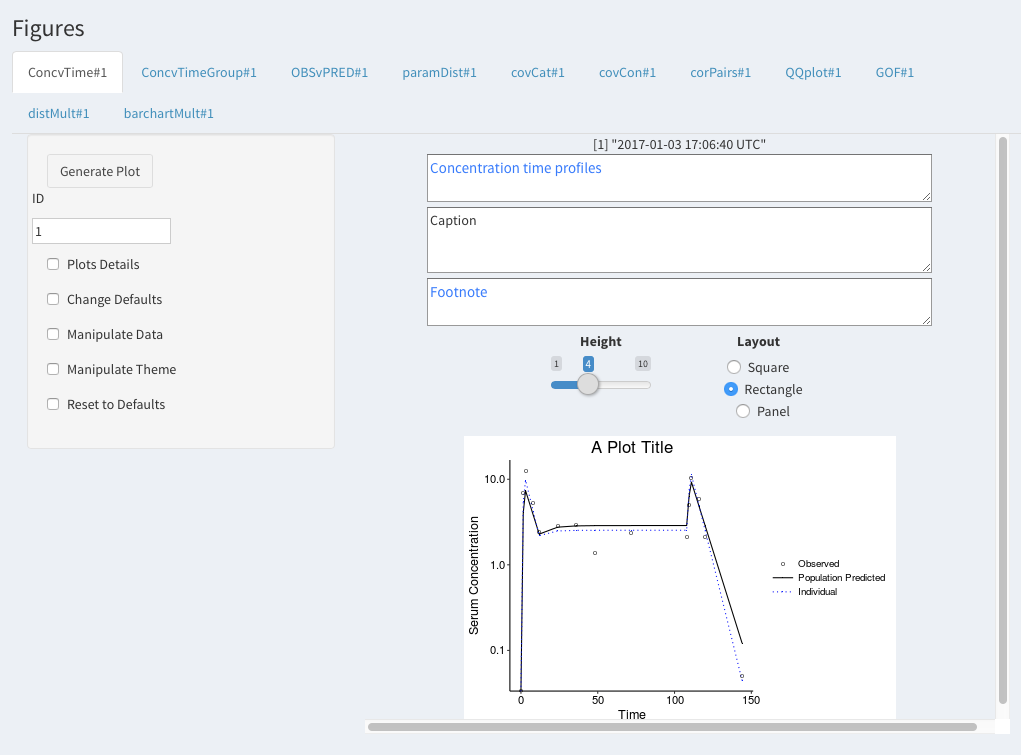
\includegraphics[width=.8\textwidth]{screencaps/01-01-1.png}
\caption{RID: 01 Test ID: 01 IDNum: 1}
\end{figure}
\begin{figure}[H]
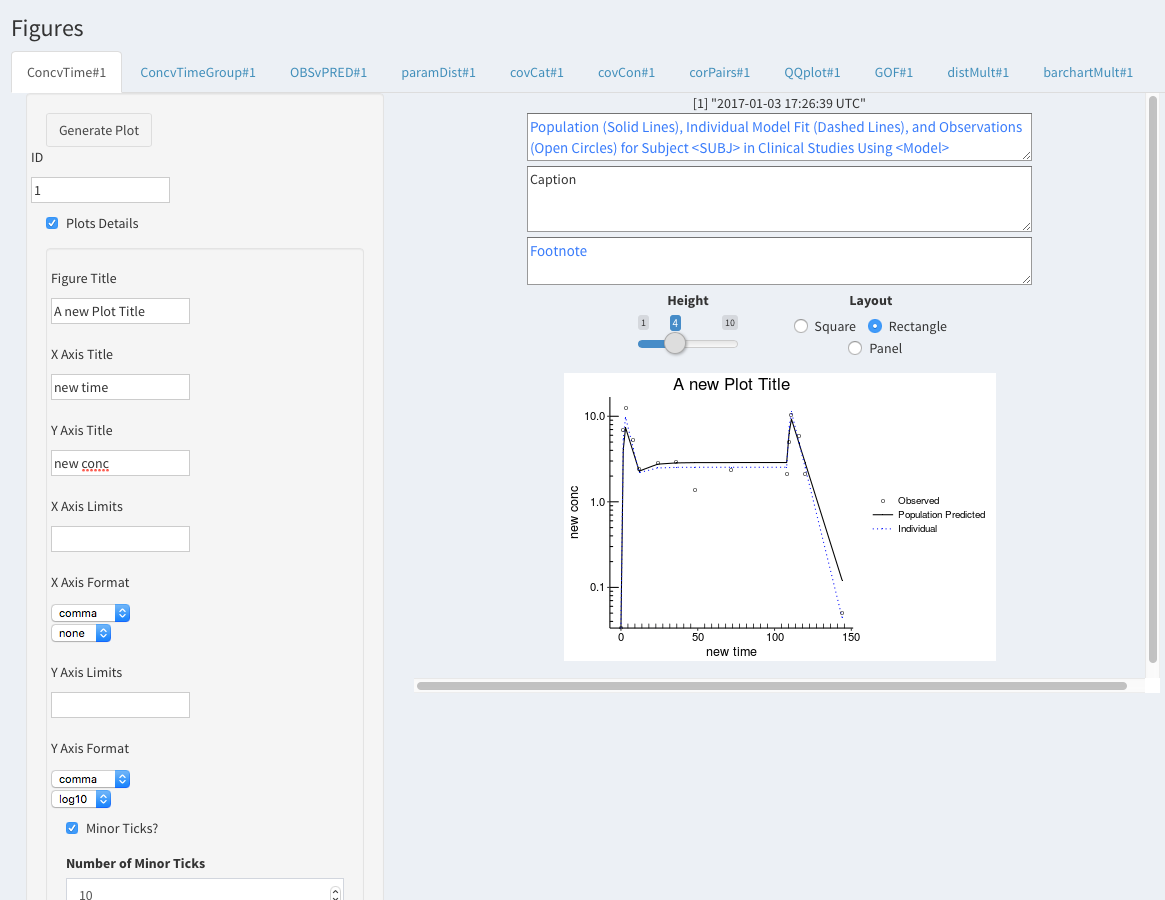
\includegraphics[width=.8\textwidth]{screencaps/01-02-1.png}
\caption{RID: 01 Test ID: 02 IDNum: 1}
\end{figure}
\begin{figure}[H]
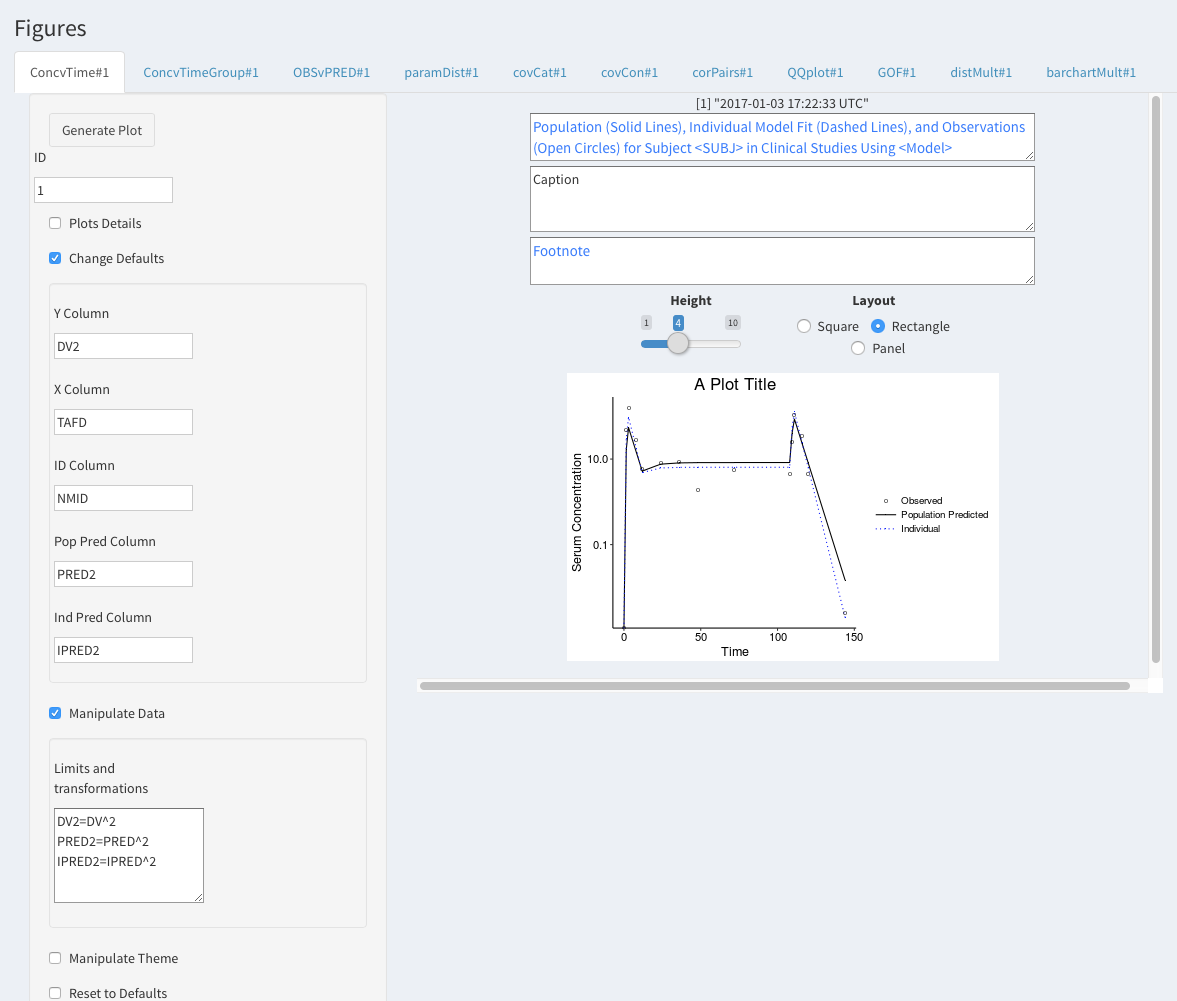
\includegraphics[width=.8\textwidth]{screencaps/01-03-1.png}
\caption{RID: 01 Test ID: 03 IDNum: 1}
\end{figure}
\begin{figure}[H]
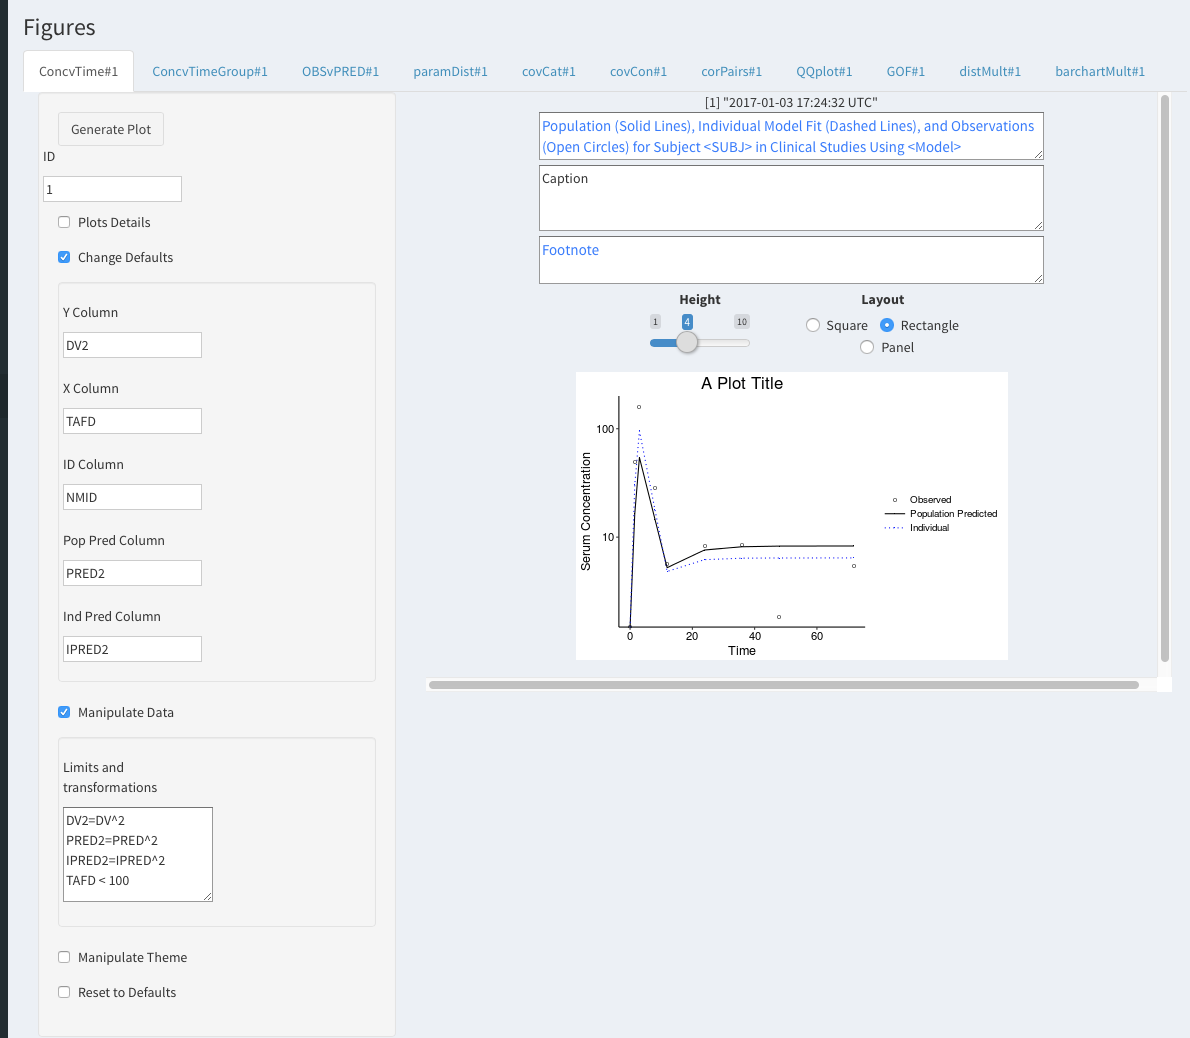
\includegraphics[width=.8\textwidth]{screencaps/01-04-1.png}
\caption{RID: 01 Test ID: 04 IDNum: 1}
\end{figure}
\begin{figure}[H]
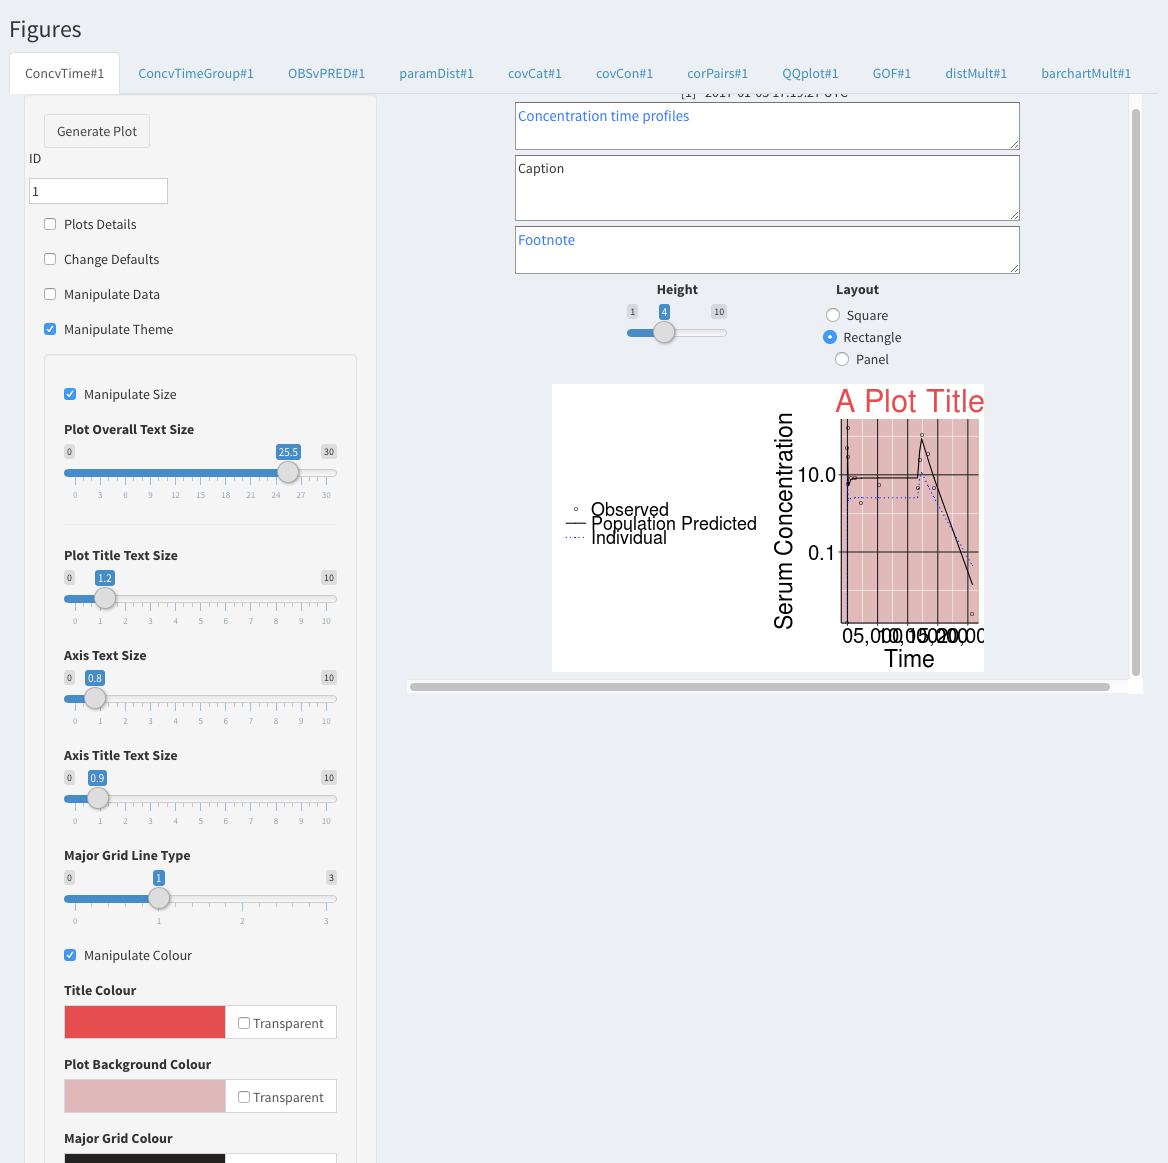
\includegraphics[width=.8\textwidth]{screencaps/01-05-1.png}
\caption{RID: 01 Test ID: 05 IDNum: 1}
\end{figure}
\begin{figure}[H]
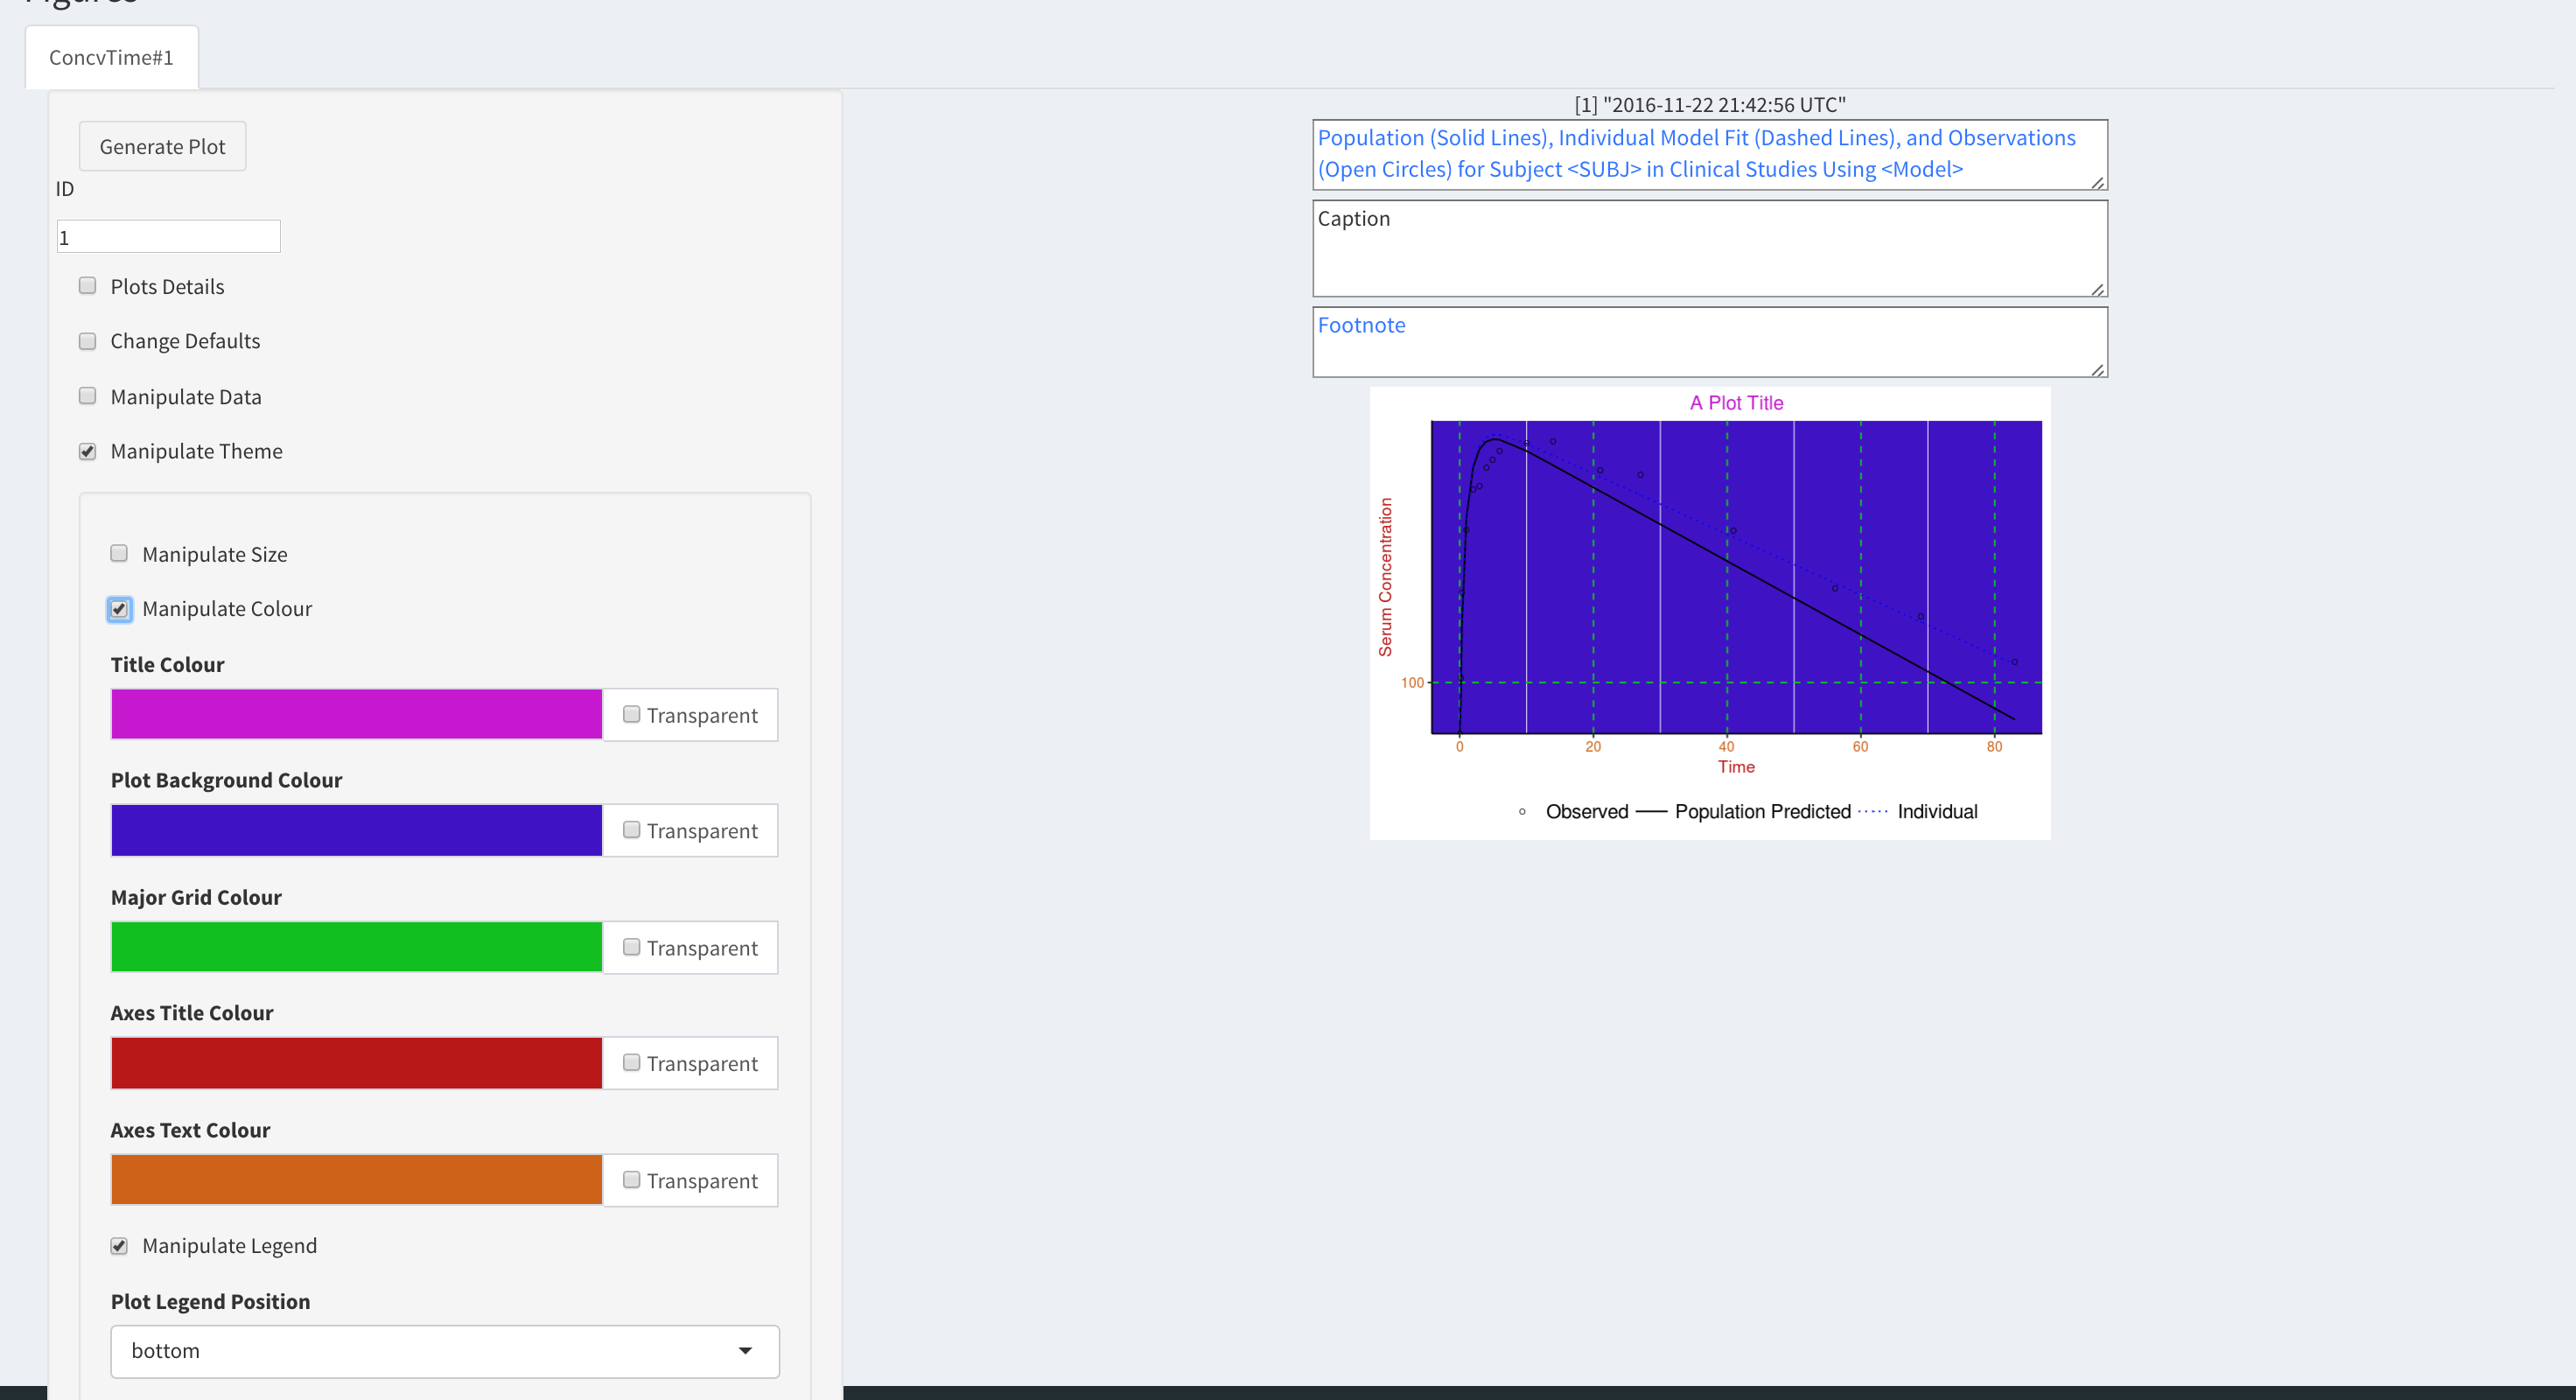
\includegraphics[width=.8\textwidth]{screencaps/01-06-1.png}
\caption{RID: 01 Test ID: 06 IDNum: 1}
\end{figure}
\begin{figure}[H]
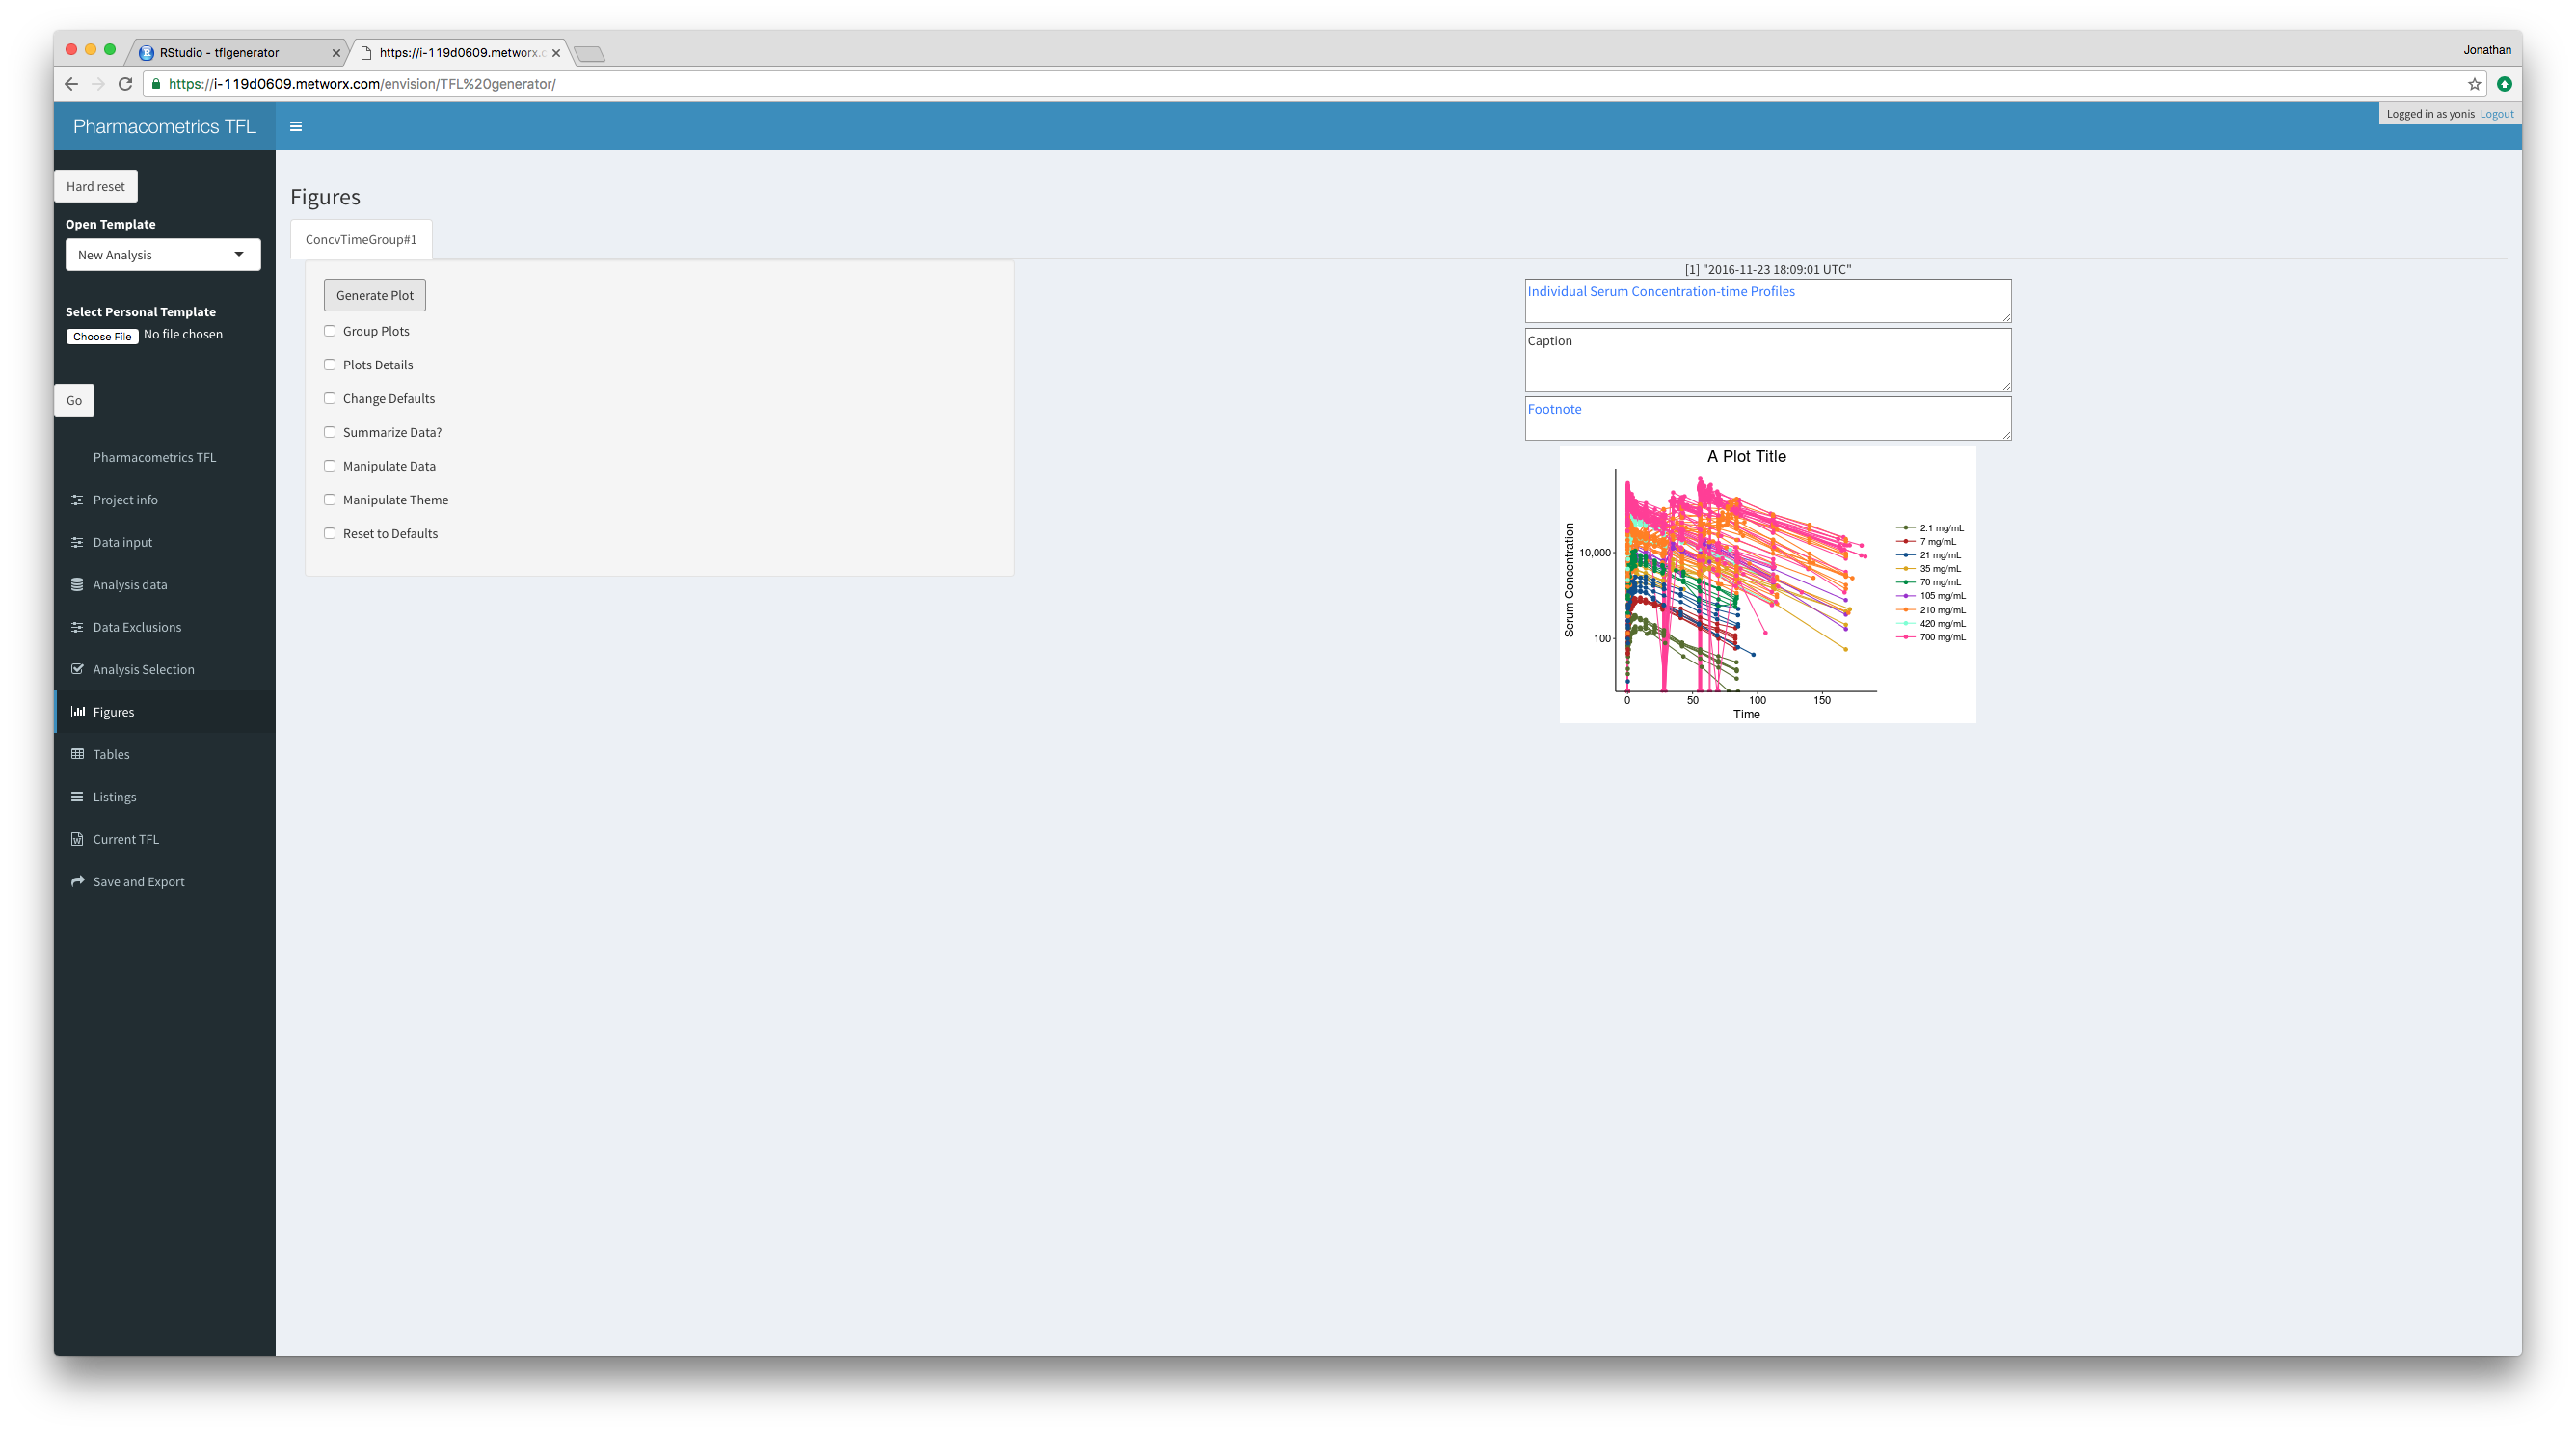
\includegraphics[width=.8\textwidth]{screencaps/02-01-1.png}
\caption{RID: 02 Test ID: 01 IDNum: 1}
\end{figure}
\begin{figure}[H]
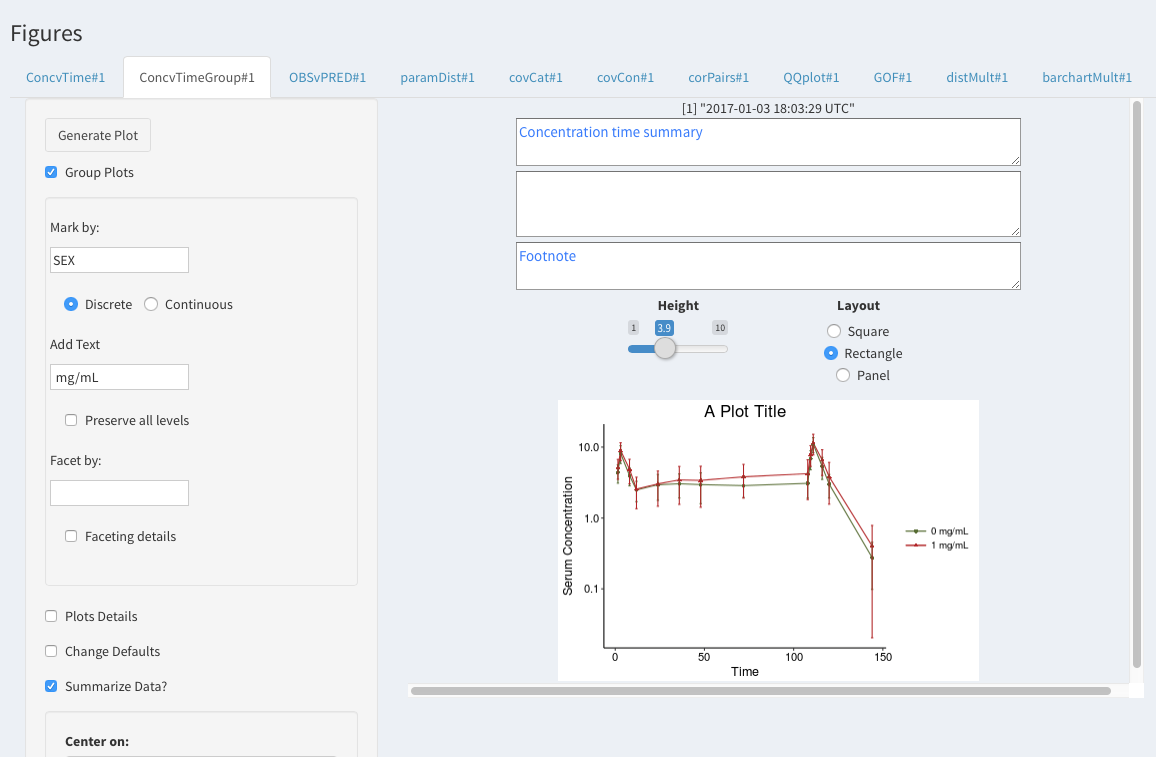
\includegraphics[width=.8\textwidth]{screencaps/02-02-1.png}
\caption{RID: 02 Test ID: 02 IDNum: 1}
\end{figure}
\begin{figure}[H]
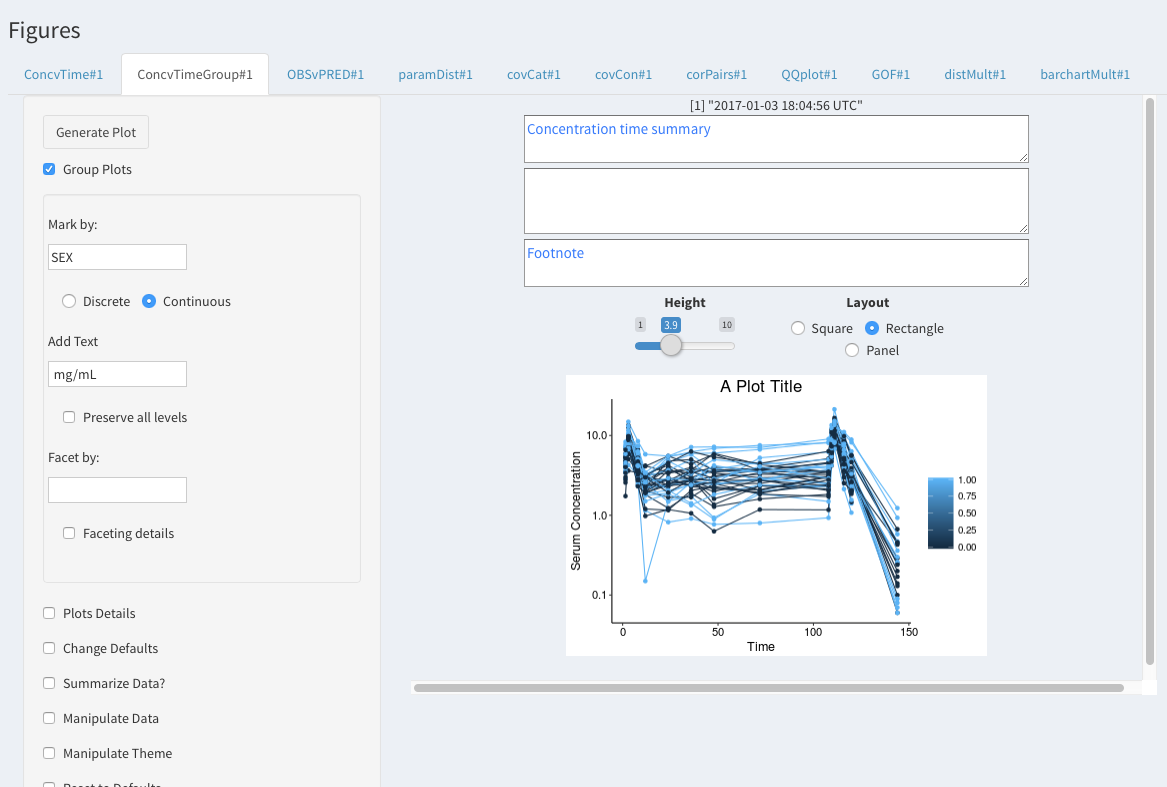
\includegraphics[width=.8\textwidth]{screencaps/02-03-1.png}
\caption{RID: 02 Test ID: 03 IDNum: 1}
\end{figure}
\begin{figure}[H]
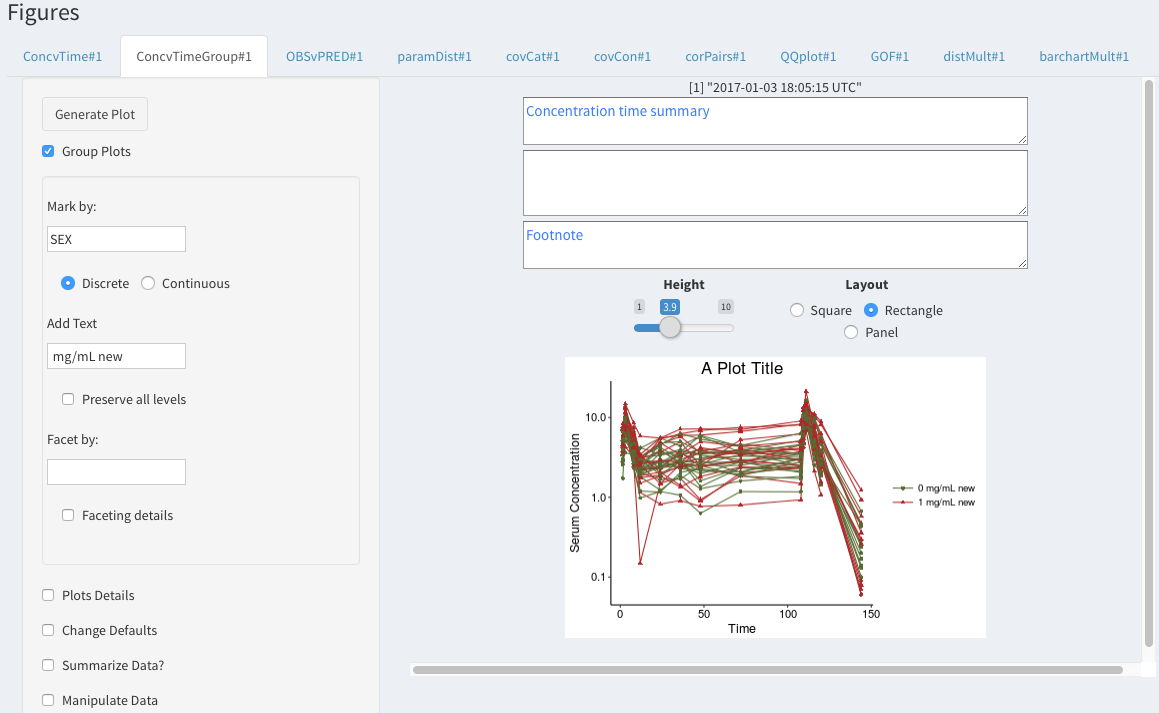
\includegraphics[width=.8\textwidth]{screencaps/02-04-1.png}
\caption{RID: 02 Test ID: 04 IDNum: 1}
\end{figure}
\begin{figure}[H]
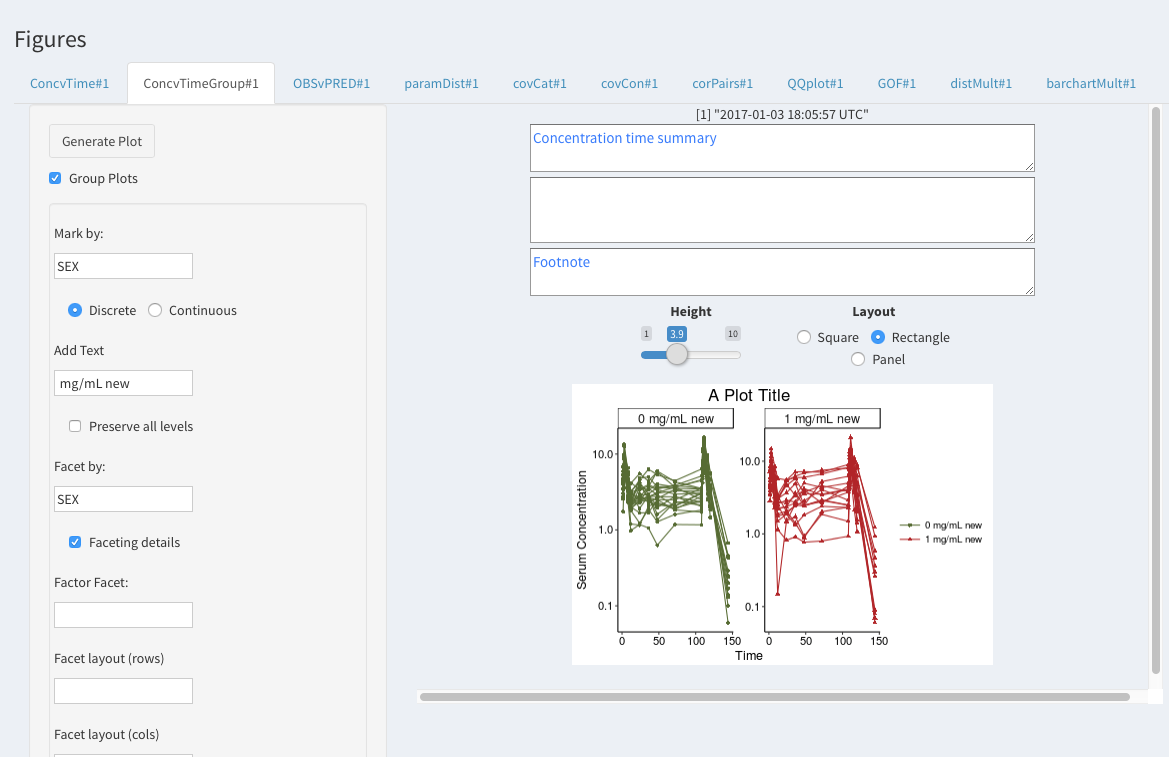
\includegraphics[width=.8\textwidth]{screencaps/02-05-1.png}
\caption{RID: 02 Test ID: 05 IDNum: 1}
\end{figure}
\begin{figure}[H]
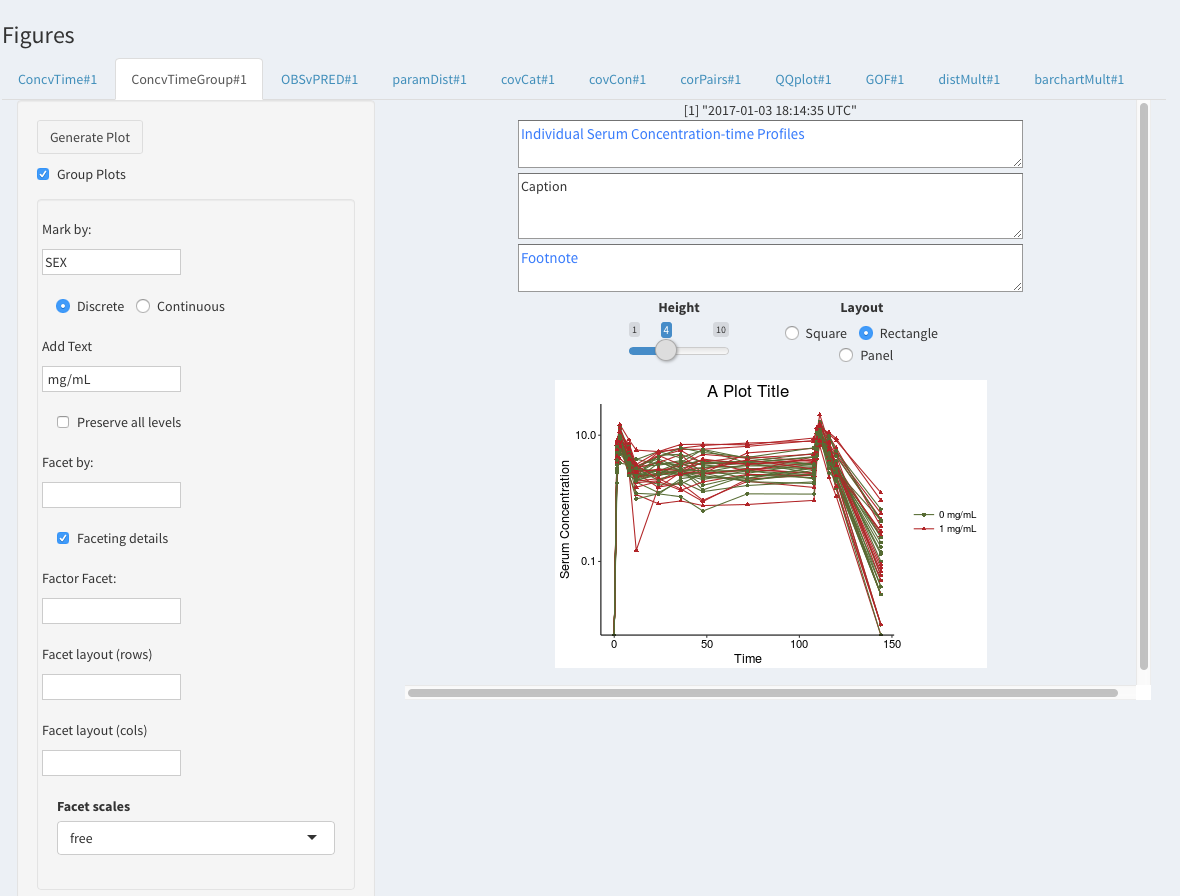
\includegraphics[width=.8\textwidth]{screencaps/02-06-1.png}
\caption{RID: 02 Test ID: 06 IDNum: 1}
\end{figure}
\begin{figure}[H]
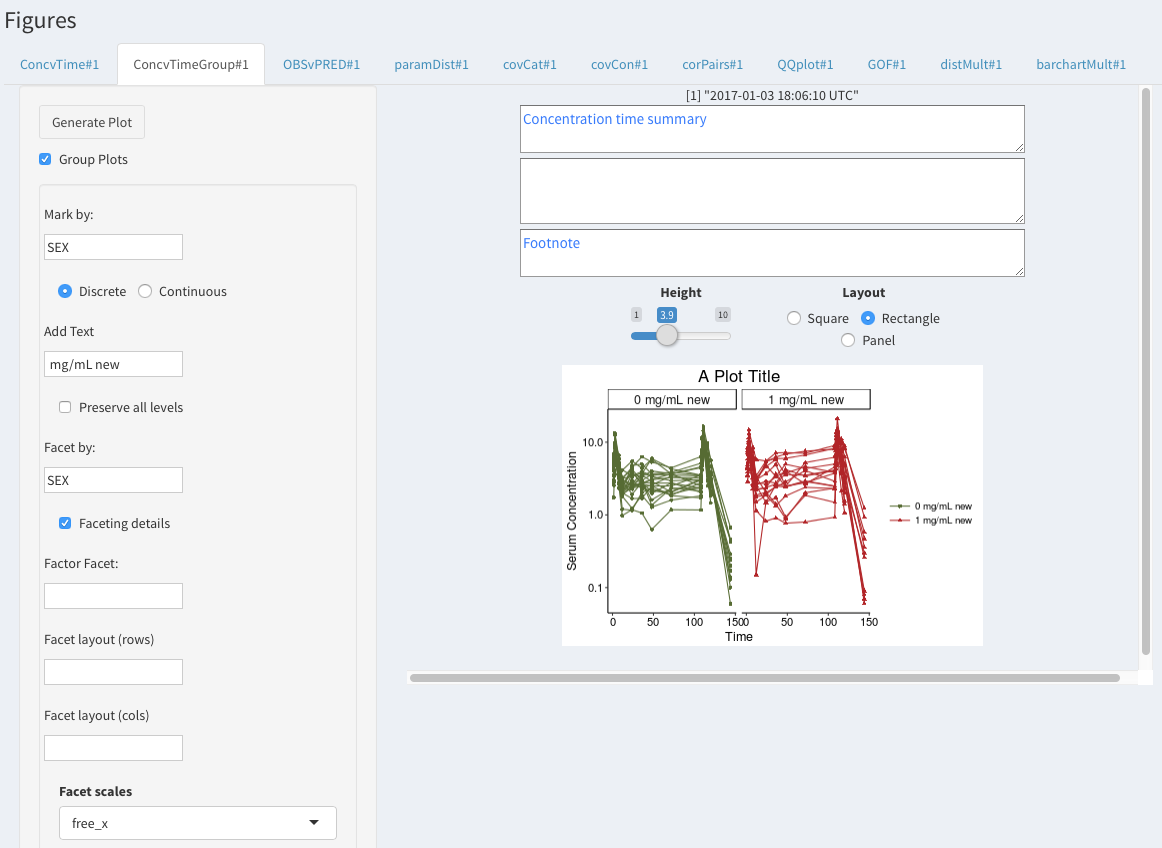
\includegraphics[width=.8\textwidth]{screencaps/02-07-1.png}
\caption{RID: 02 Test ID: 07 IDNum: 1}
\end{figure}
\begin{figure}[H]
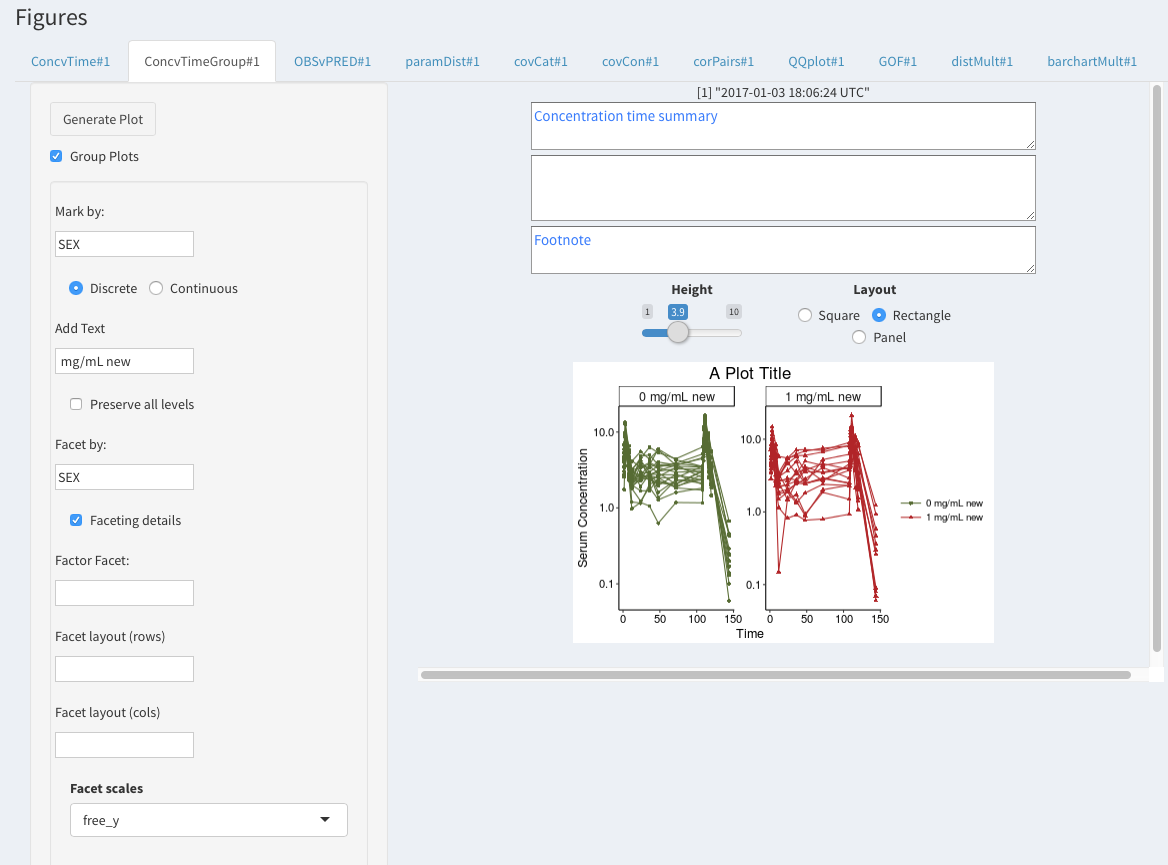
\includegraphics[width=.8\textwidth]{screencaps/02-08-1.png}
\caption{RID: 02 Test ID: 08 IDNum: 1}
\end{figure}
\begin{figure}[H]
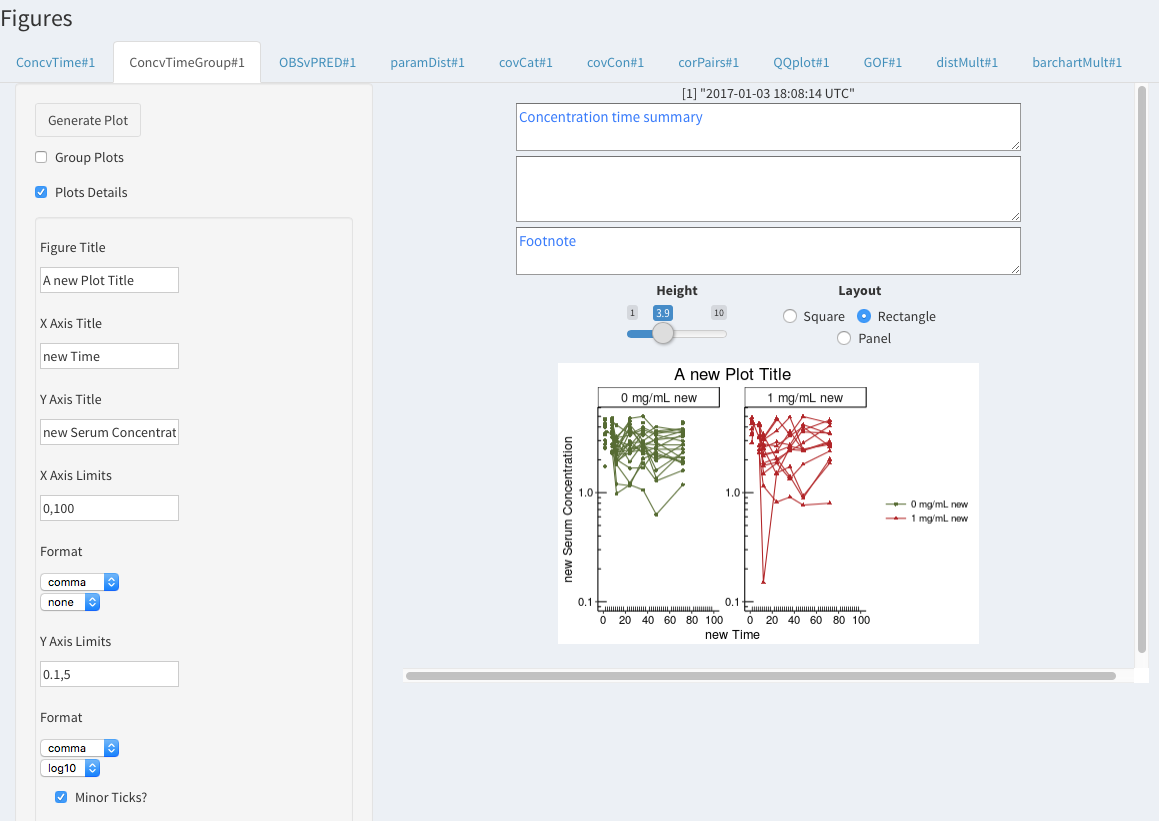
\includegraphics[width=.8\textwidth]{screencaps/02-09-1.png}
\caption{RID: 02 Test ID: 09 IDNum: 1}
\end{figure}
\begin{figure}[H]
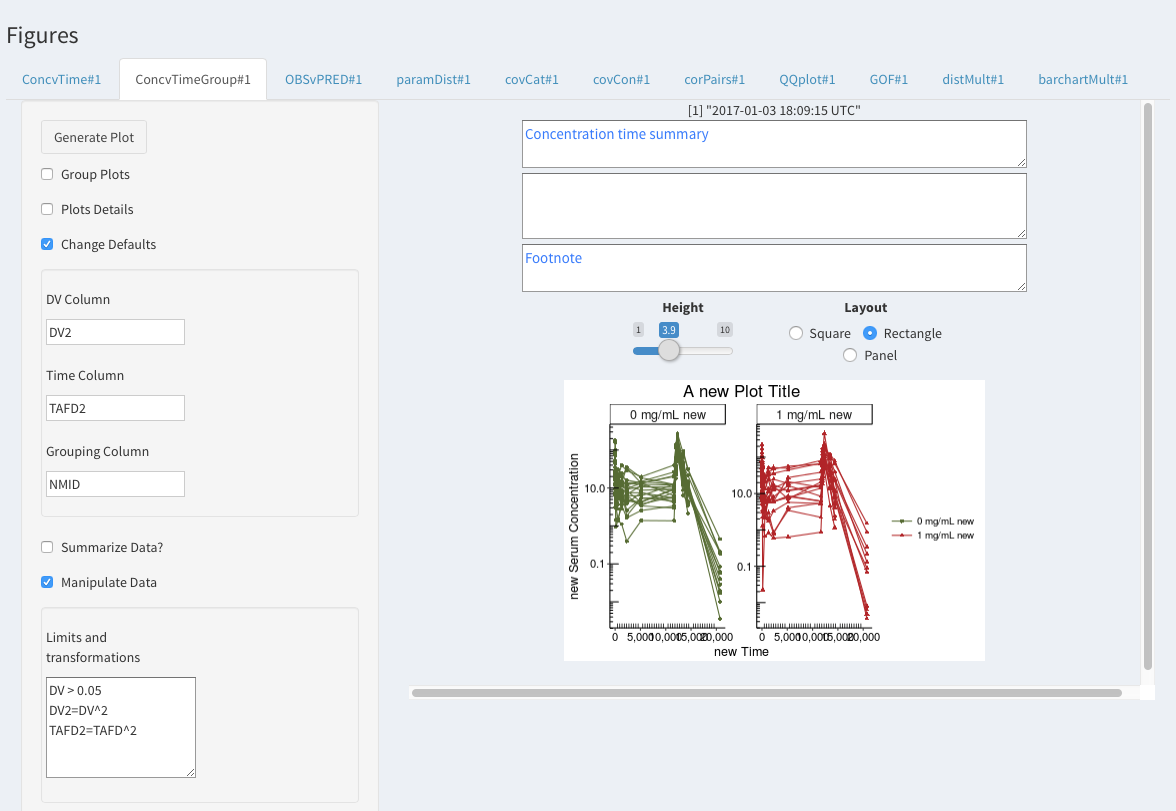
\includegraphics[width=.8\textwidth]{screencaps/02-10-1.png}
\caption{RID: 02 Test ID: 10 IDNum: 1}
\end{figure}
\begin{figure}[H]
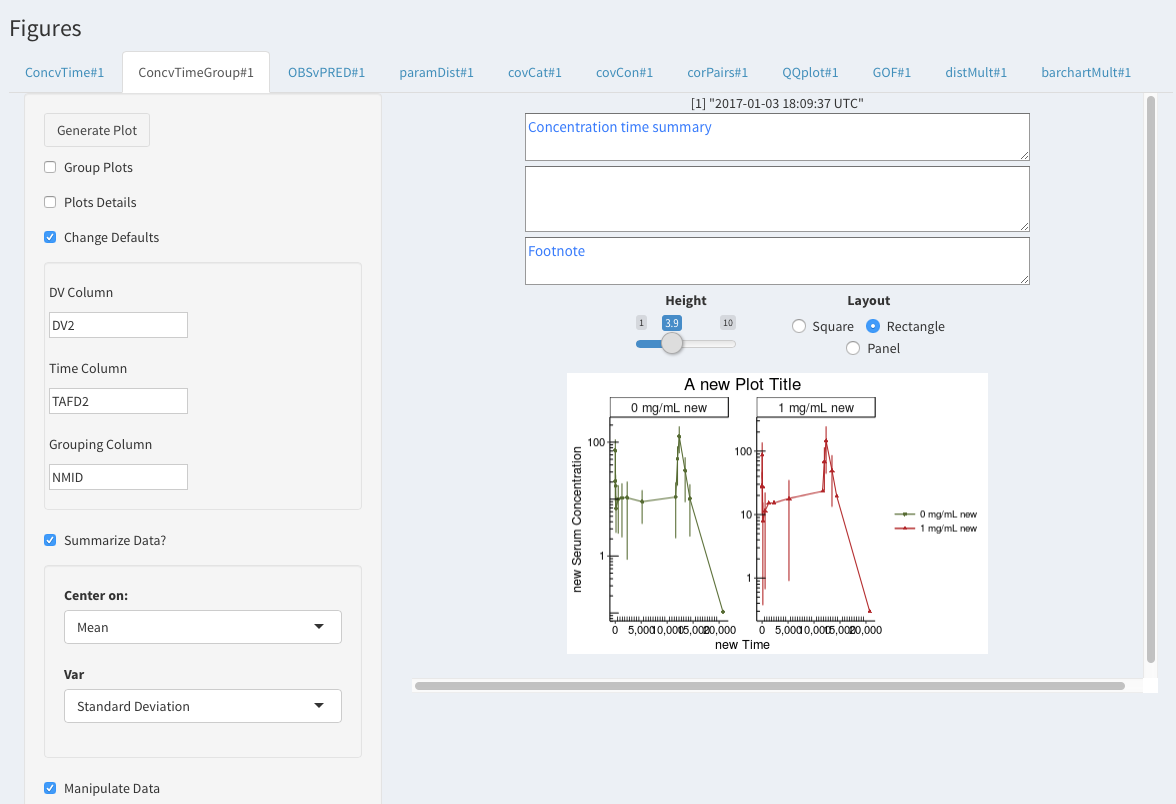
\includegraphics[width=.8\textwidth]{screencaps/02-11-1.png}
\caption{RID: 02 Test ID: 11 IDNum: 1}
\end{figure}
\begin{figure}[H]
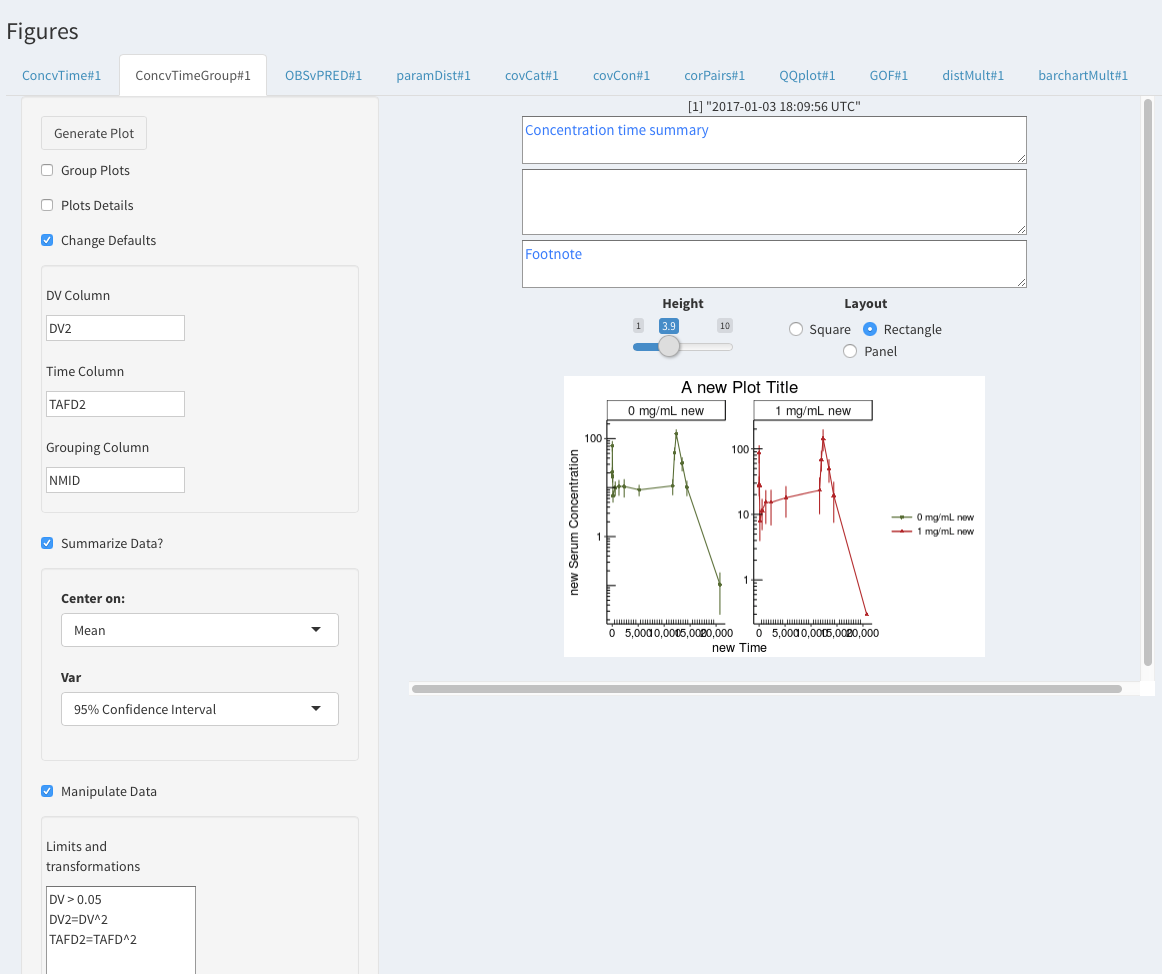
\includegraphics[width=.8\textwidth]{screencaps/02-12-1.png}
\caption{RID: 02 Test ID: 12 IDNum: 1}
\end{figure}
\begin{figure}[H]
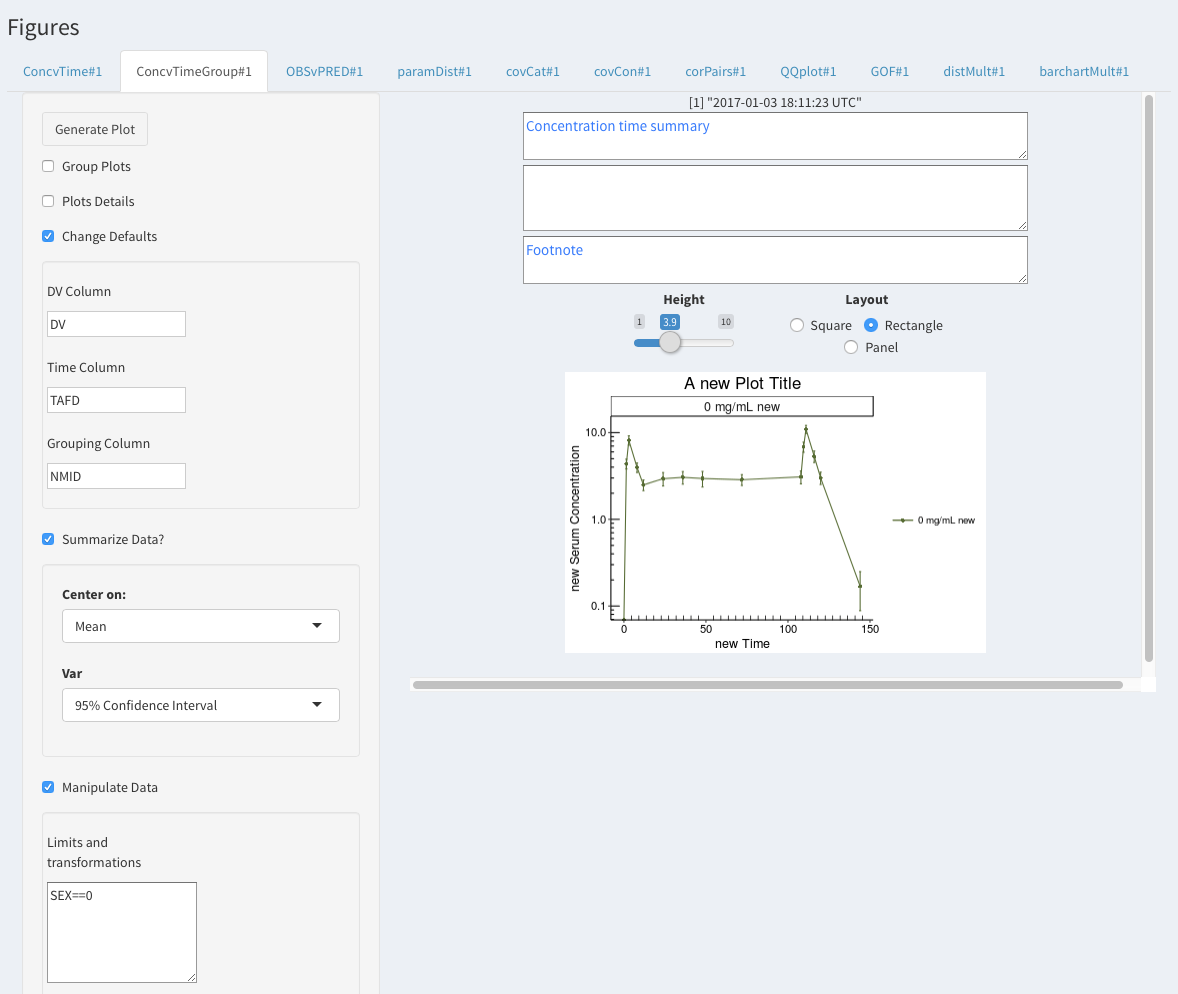
\includegraphics[width=.8\textwidth]{screencaps/02-13-1.png}
\caption{RID: 02 Test ID: 13 IDNum: 1}
\end{figure}
\begin{figure}[H]
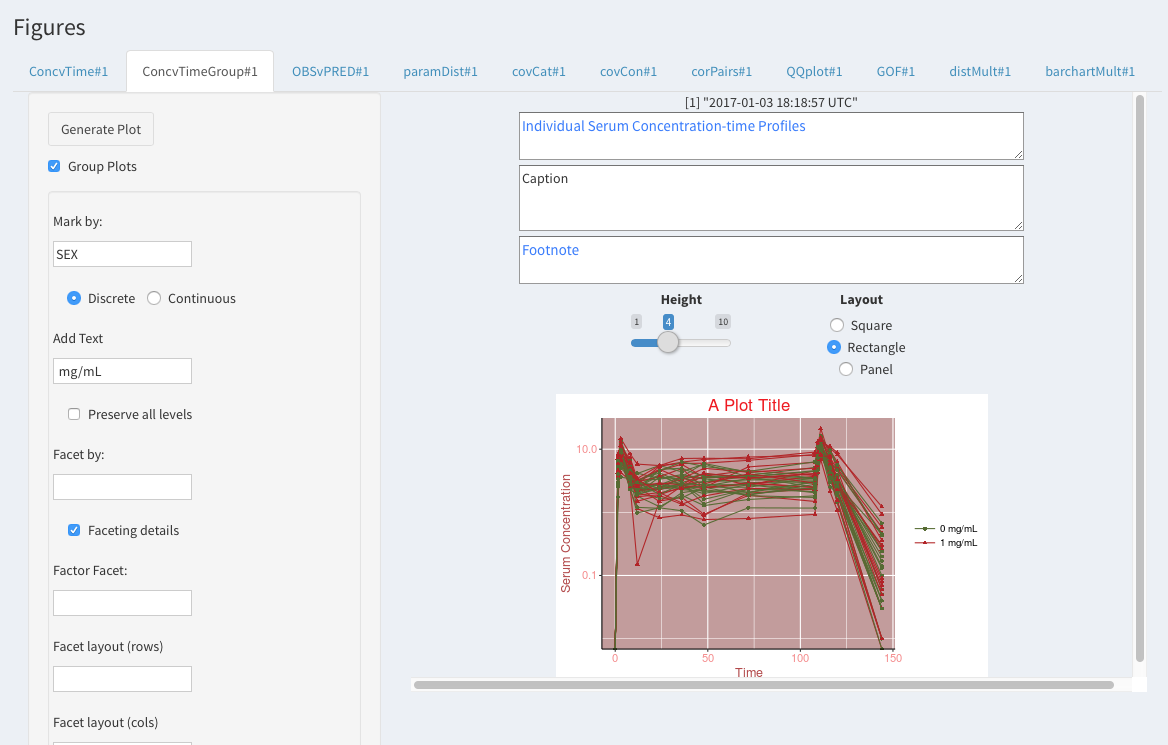
\includegraphics[width=.8\textwidth]{screencaps/02-15-1.png}
\caption{RID: 02 Test ID: 15 IDNum: 1}
\end{figure}
\begin{figure}[H]
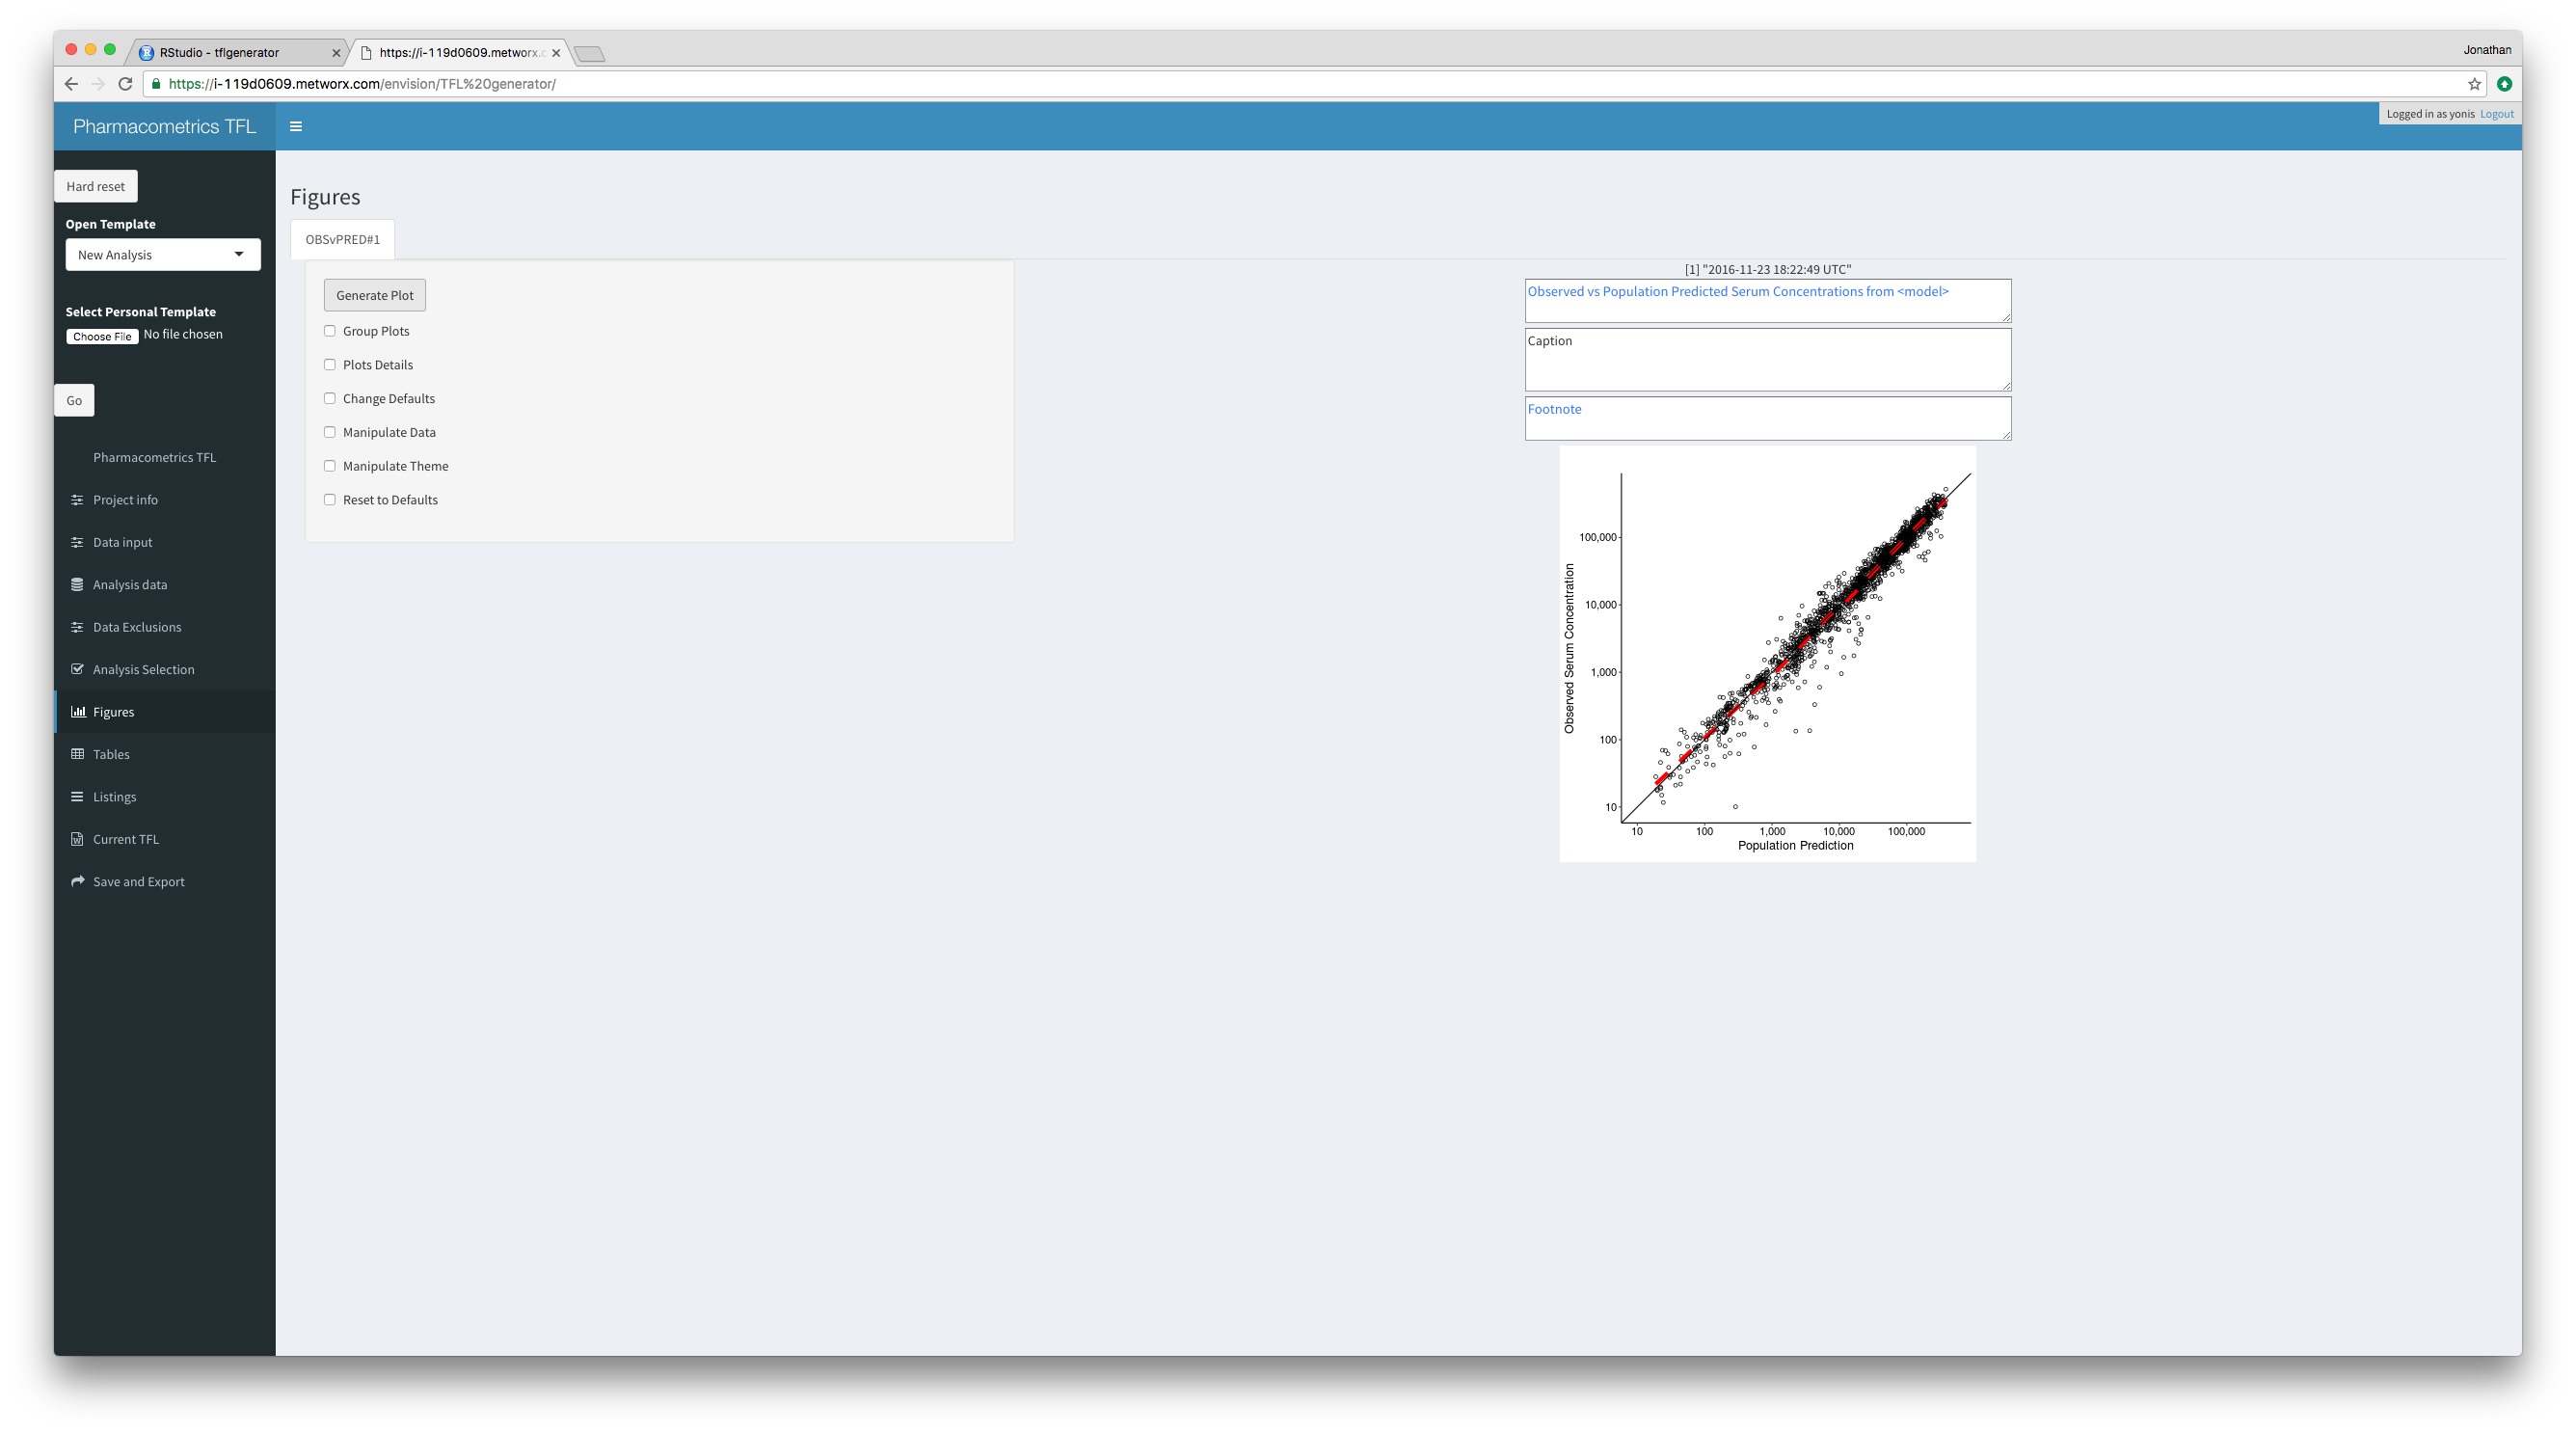
\includegraphics[width=.8\textwidth]{screencaps/03-01-1.png}
\caption{RID: 03 Test ID: 01 IDNum: 1}
\end{figure}
\begin{figure}[H]
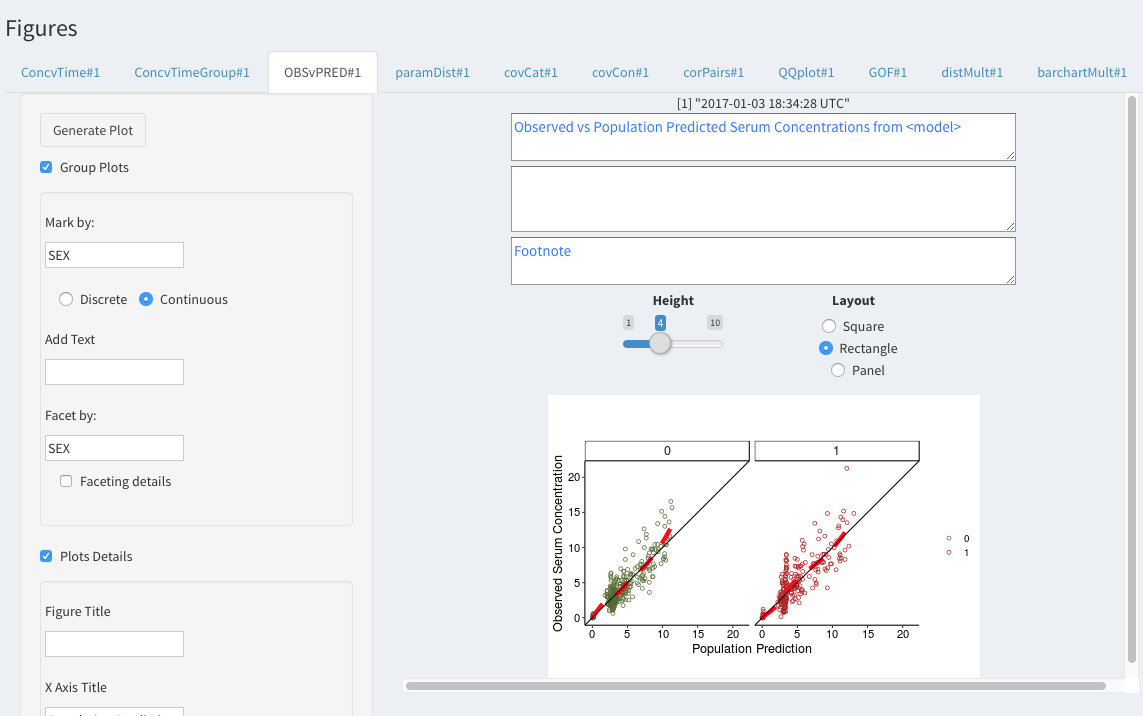
\includegraphics[width=.8\textwidth]{screencaps/03-02-1.png}
\caption{RID: 03 Test ID: 02 IDNum: 1}
\end{figure}
\begin{figure}[H]
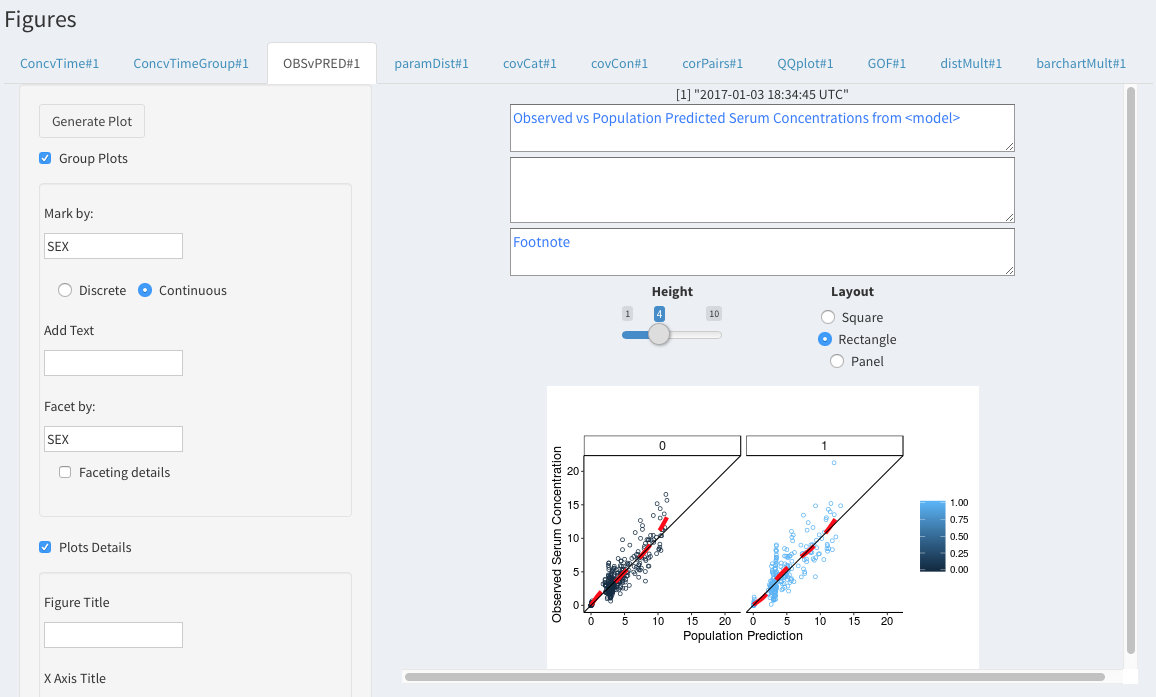
\includegraphics[width=.8\textwidth]{screencaps/03-03-1.png}
\caption{RID: 03 Test ID: 03 IDNum: 1}
\end{figure}
\begin{figure}[H]
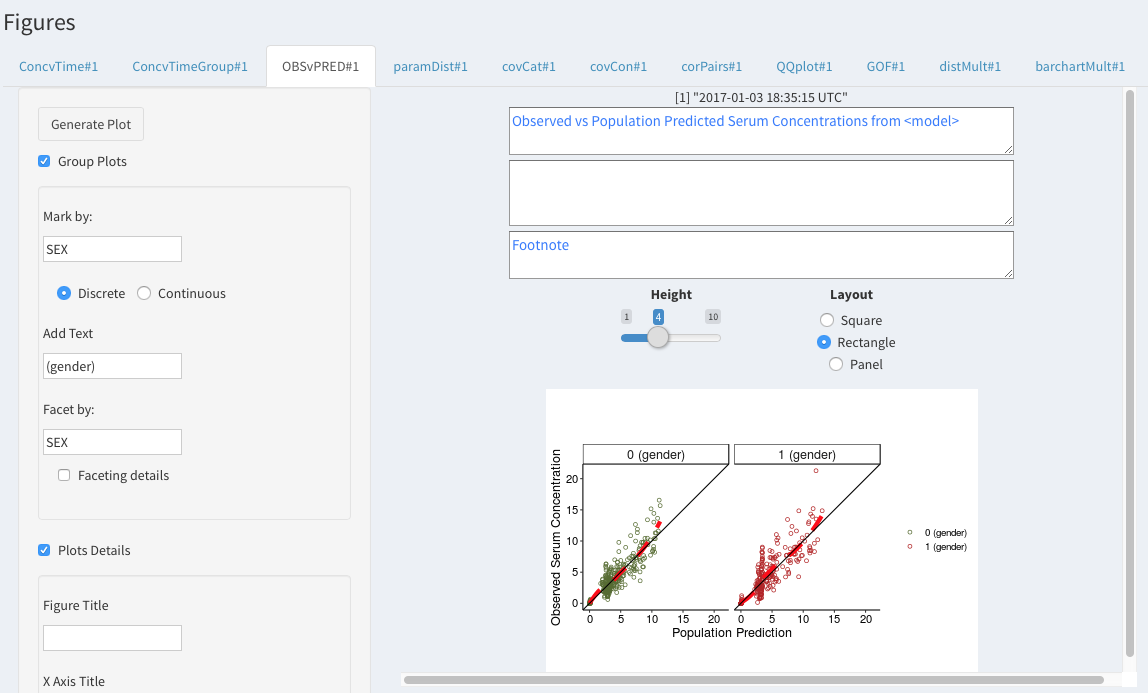
\includegraphics[width=.8\textwidth]{screencaps/03-04-1.png}
\caption{RID: 03 Test ID: 04 IDNum: 1}
\end{figure}
\begin{figure}[H]
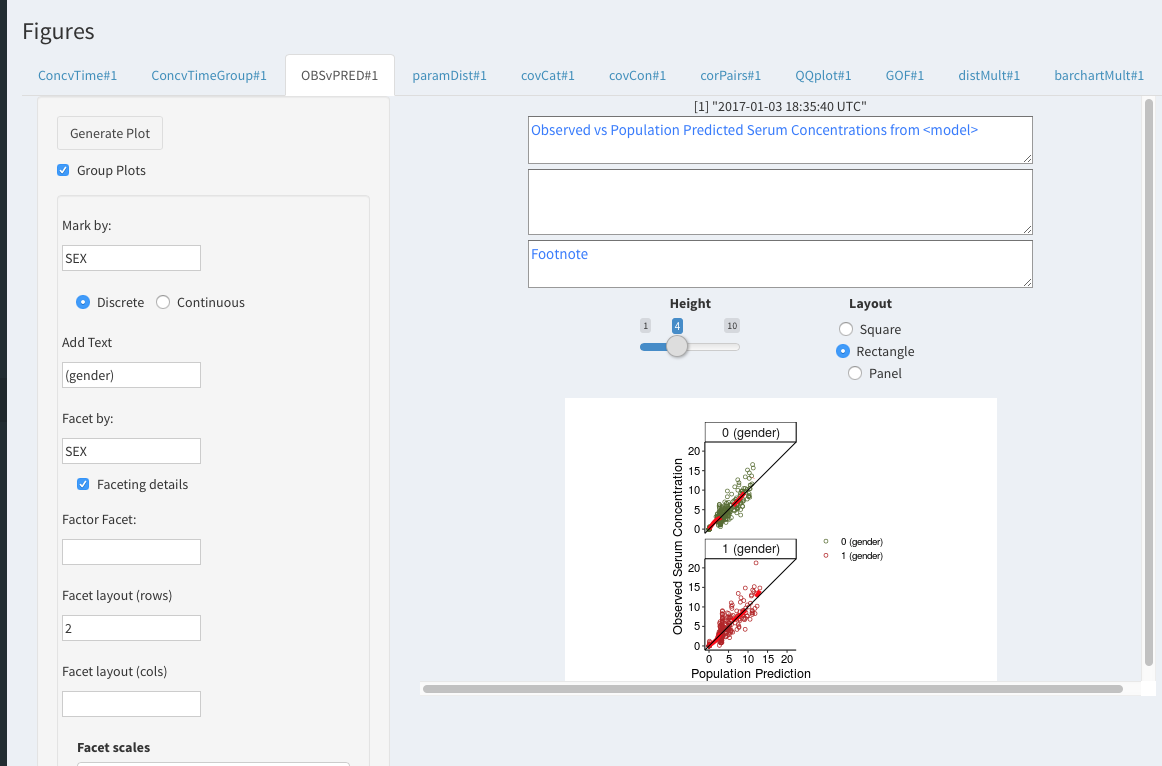
\includegraphics[width=.8\textwidth]{screencaps/03-05-1.png}
\caption{RID: 03 Test ID: 05 IDNum: 1}
\end{figure}
\begin{figure}[H]
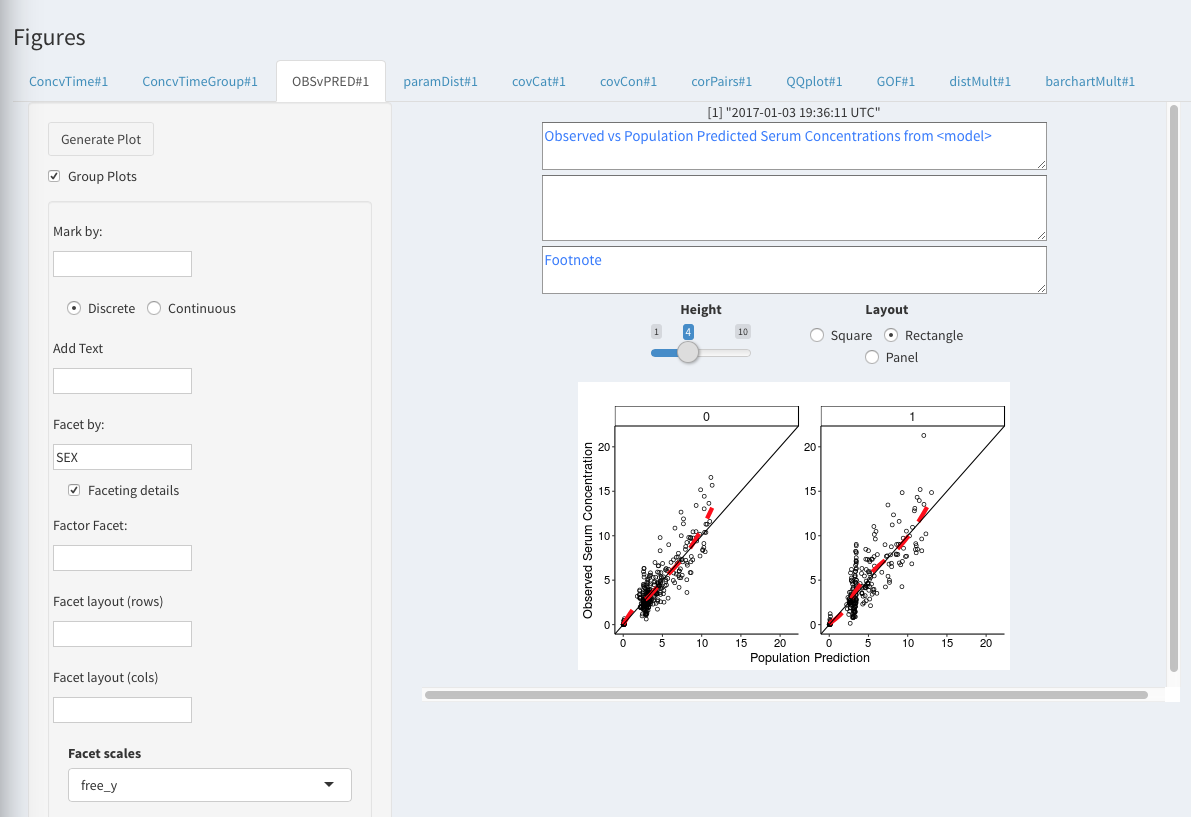
\includegraphics[width=.8\textwidth]{screencaps/03-06-1.png}
\caption{RID: 03 Test ID: 06 IDNum: 1}
\end{figure}
\begin{figure}[H]
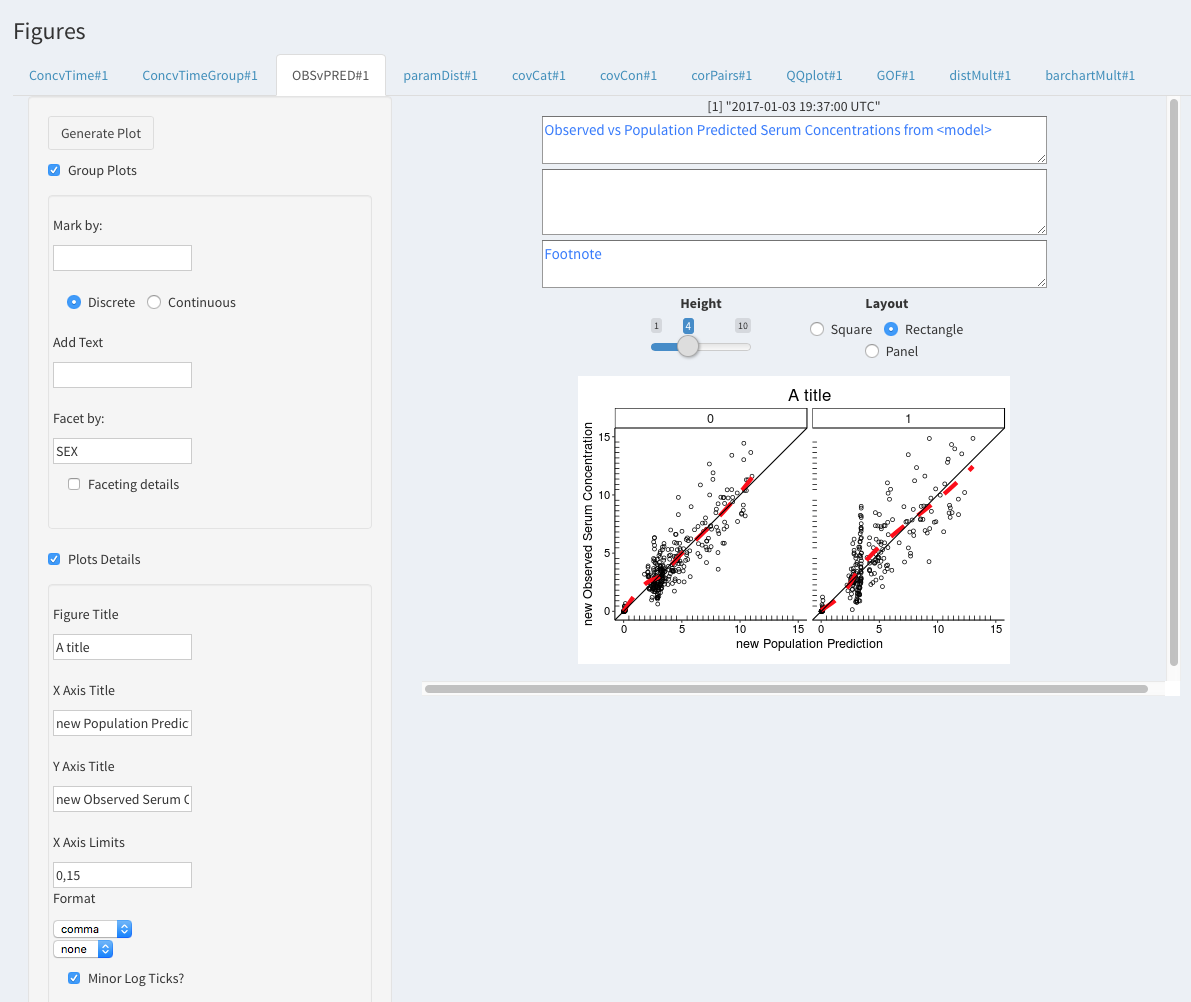
\includegraphics[width=.8\textwidth]{screencaps/03-07-1.png}
\caption{RID: 03 Test ID: 07 IDNum: 1}
\end{figure}
\begin{figure}[H]
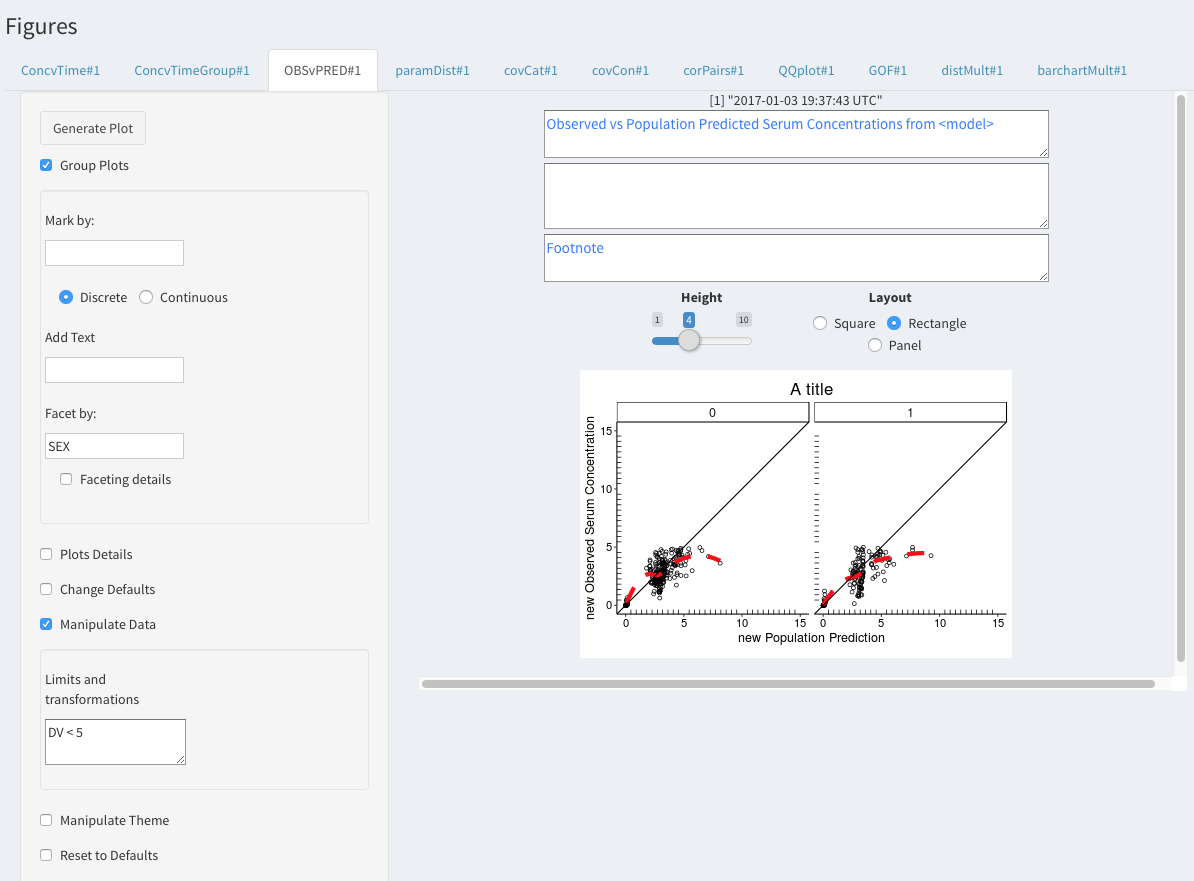
\includegraphics[width=.8\textwidth]{screencaps/03-08-1.png}
\caption{RID: 03 Test ID: 08 IDNum: 1}
\end{figure}
\begin{figure}[H]
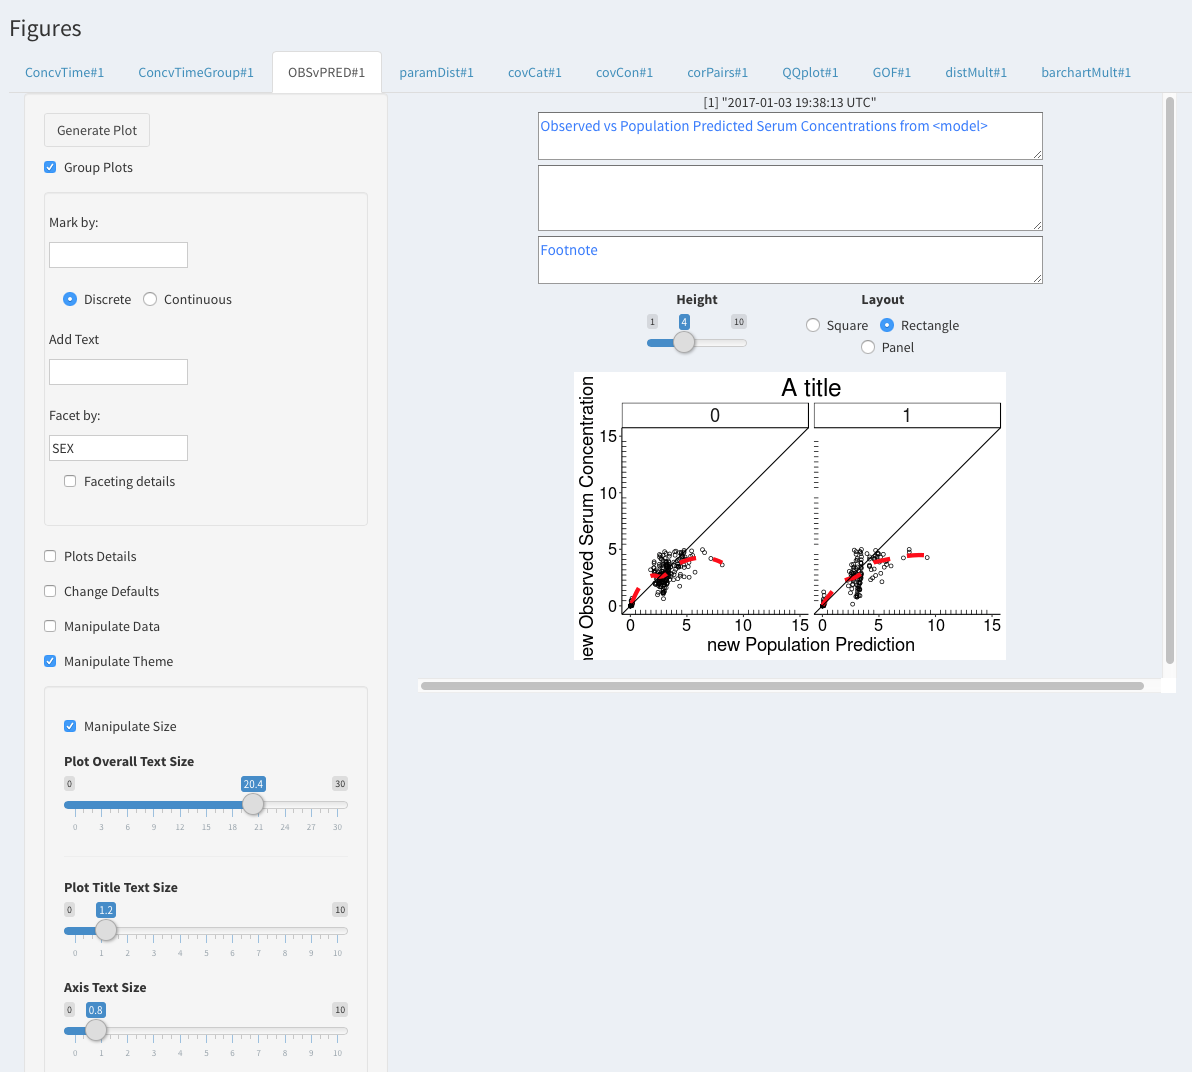
\includegraphics[width=.8\textwidth]{screencaps/03-09-1.png}
\caption{RID: 03 Test ID: 09 IDNum: 1}
\end{figure}
\begin{figure}[H]
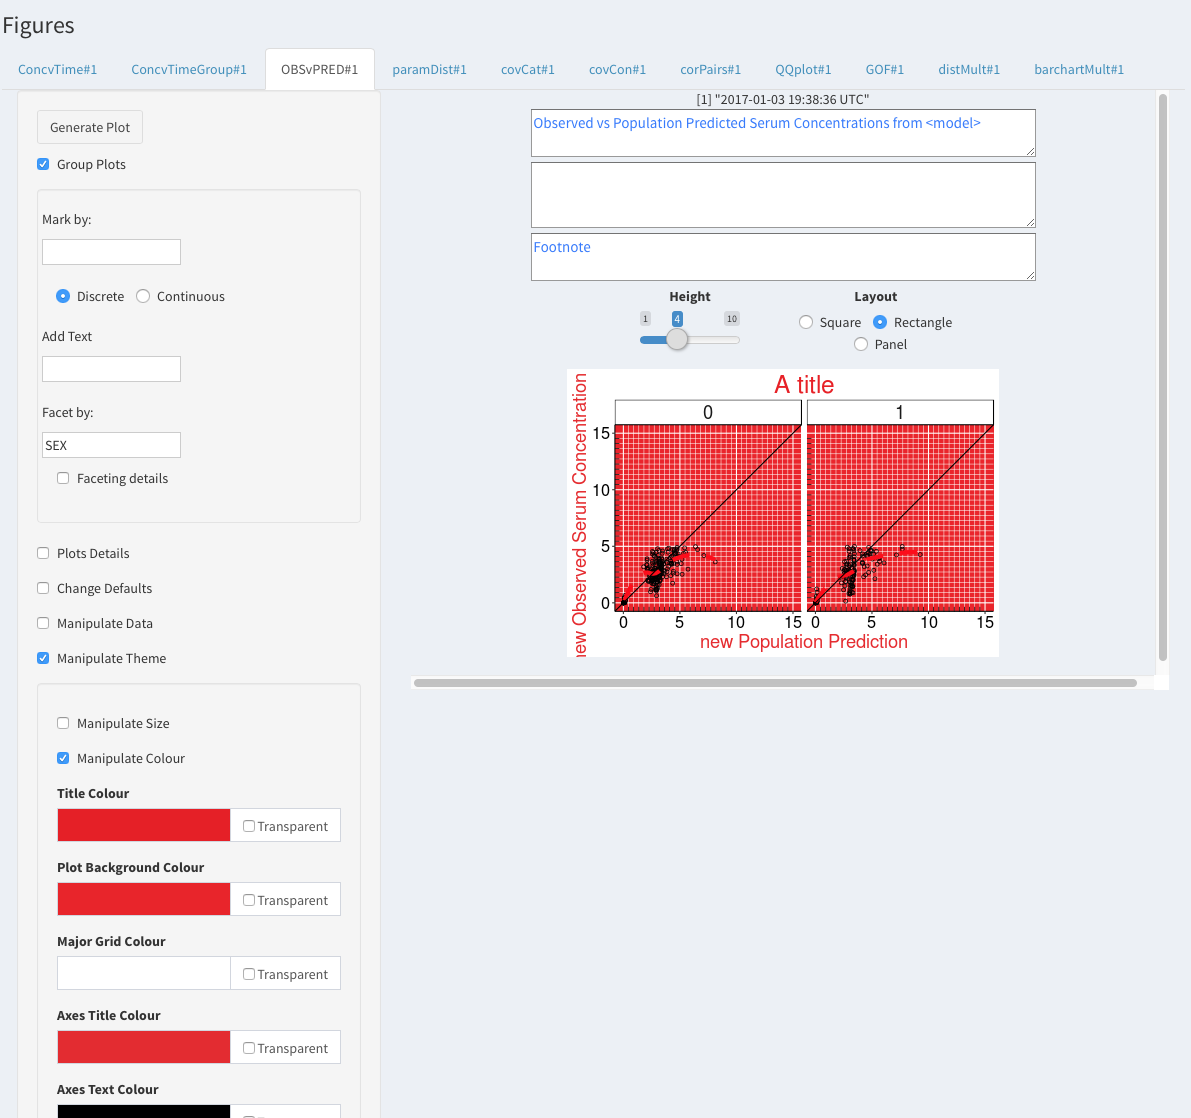
\includegraphics[width=.8\textwidth]{screencaps/03-10-1.png}
\caption{RID: 03 Test ID: 10 IDNum: 1}
\end{figure}
\begin{figure}[H]
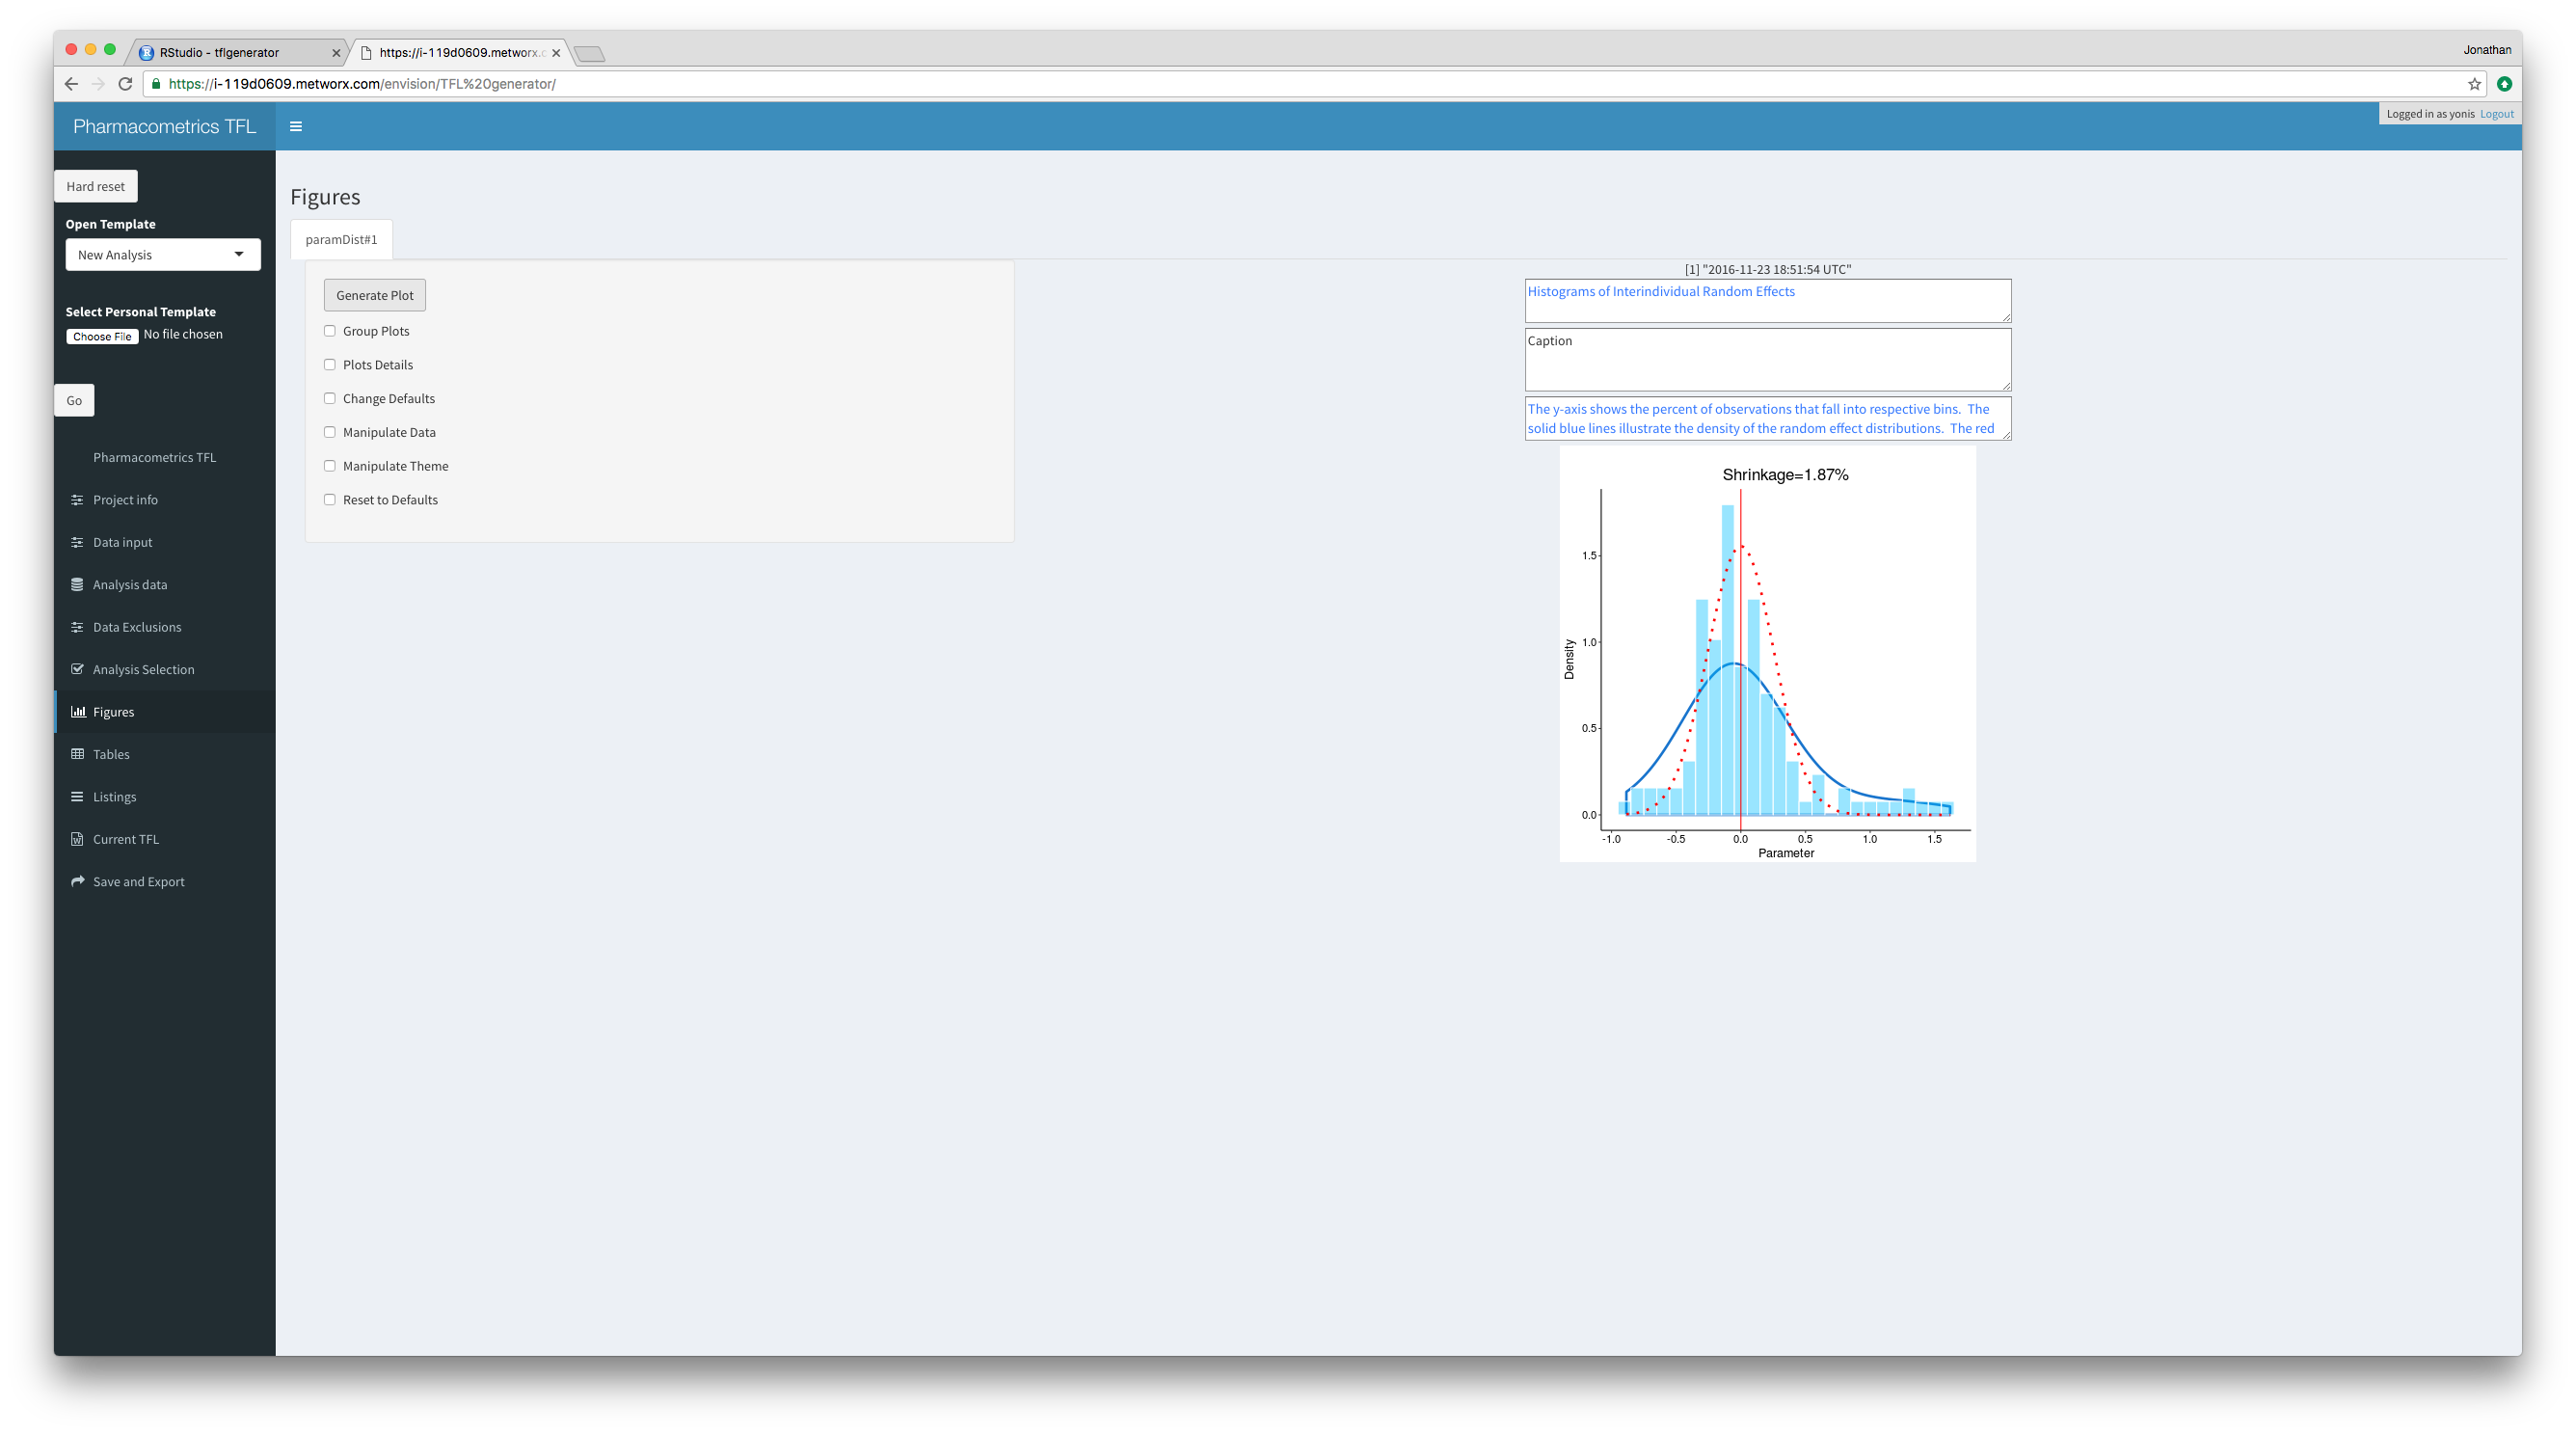
\includegraphics[width=.8\textwidth]{screencaps/04-01-1.png}
\caption{RID: 04 Test ID: 01 IDNum: 1}
\end{figure}
\begin{figure}[H]
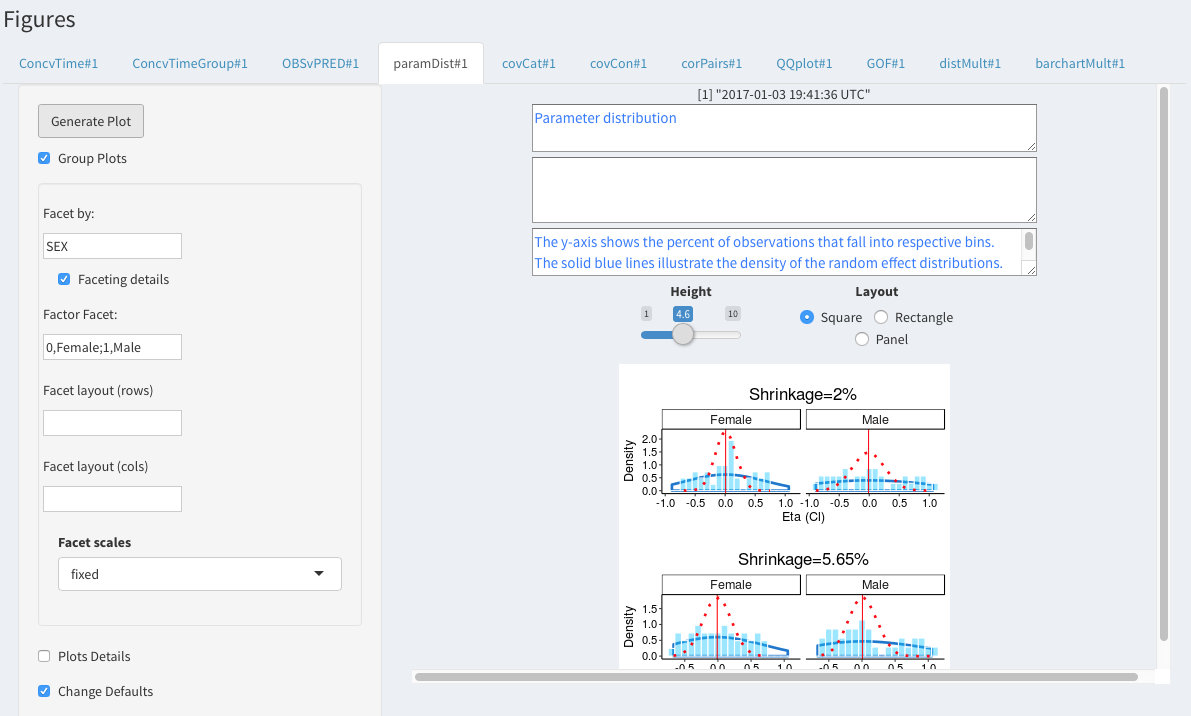
\includegraphics[width=.8\textwidth]{screencaps/04-02-1.png}
\caption{RID: 04 Test ID: 02 IDNum: 1}
\end{figure}
\begin{figure}[H]
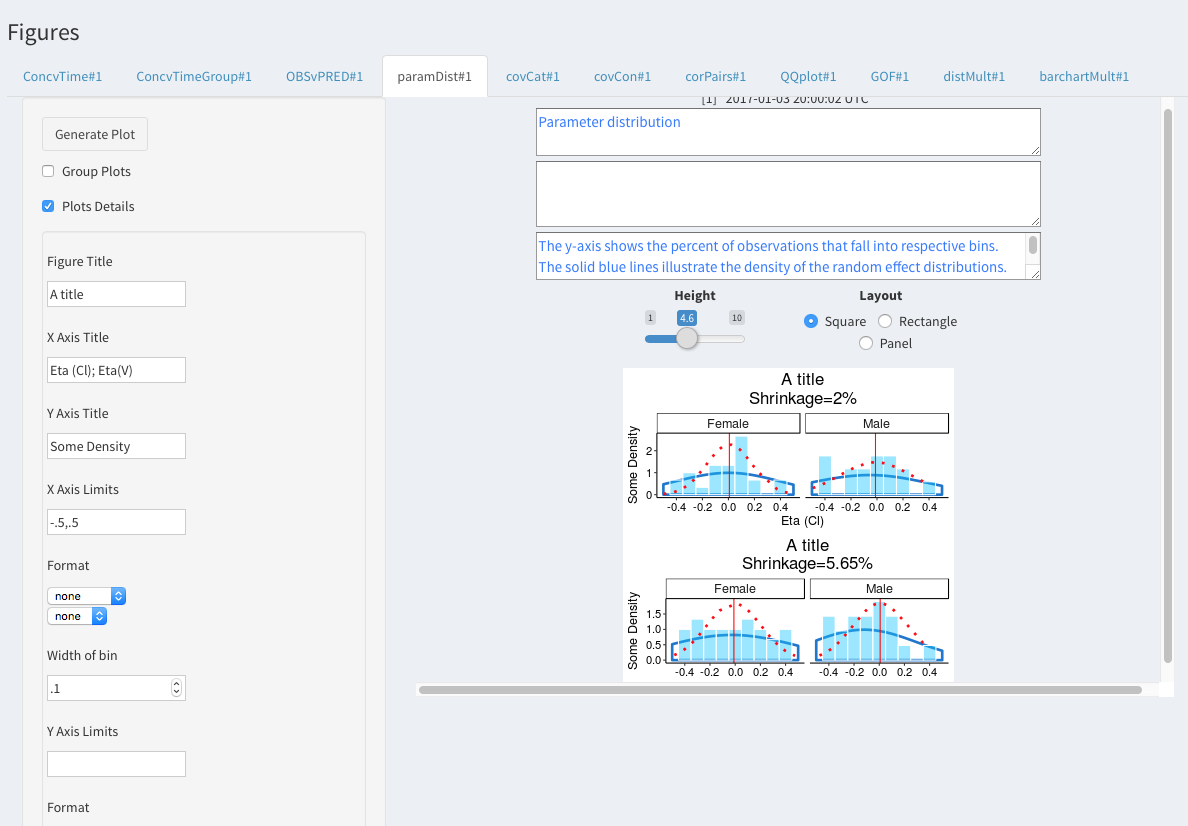
\includegraphics[width=.8\textwidth]{screencaps/04-03-1.png}
\caption{RID: 04 Test ID: 03 IDNum: 1}
\end{figure}
\begin{figure}[H]
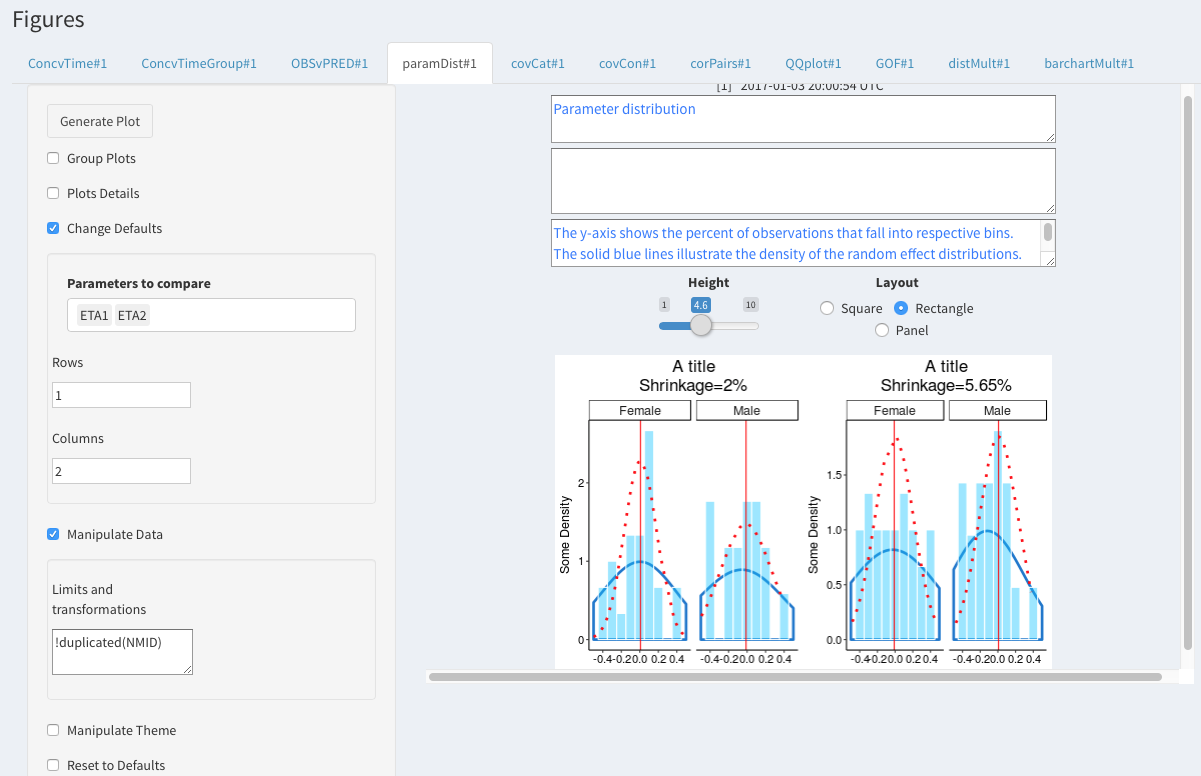
\includegraphics[width=.8\textwidth]{screencaps/04-04-1.png}
\caption{RID: 04 Test ID: 04 IDNum: 1}
\end{figure}
\begin{figure}[H]
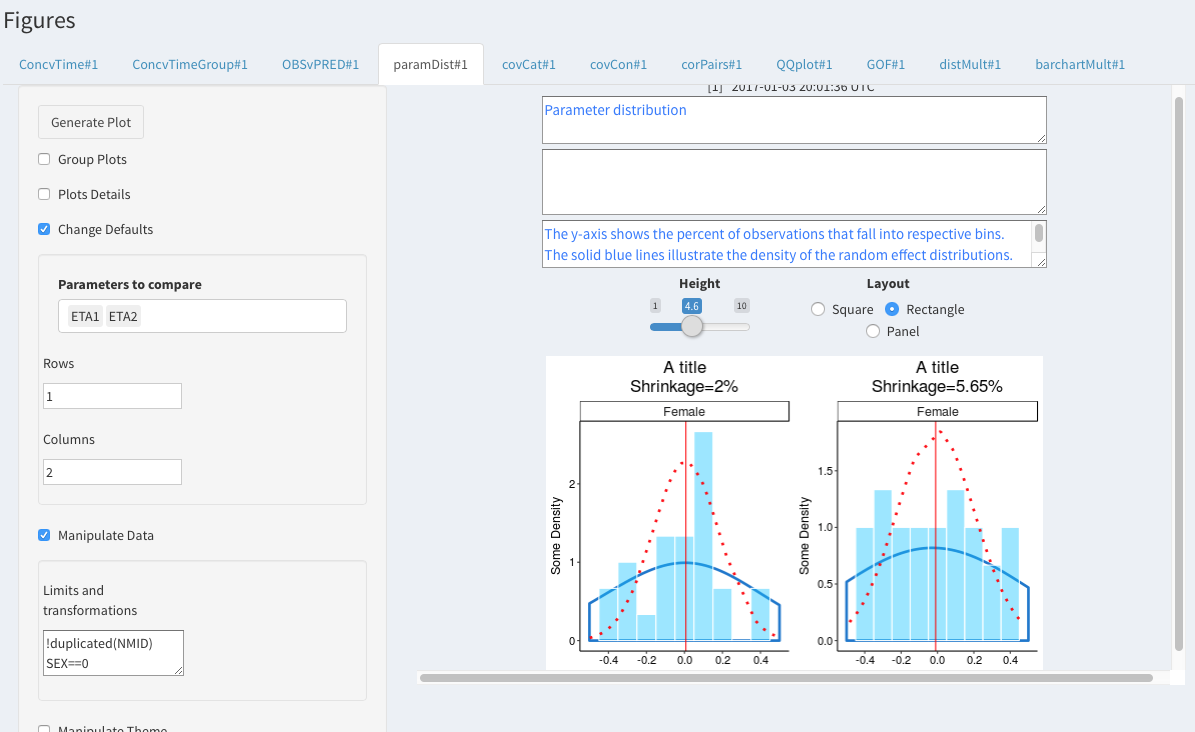
\includegraphics[width=.8\textwidth]{screencaps/04-05-1.png}
\caption{RID: 04 Test ID: 05 IDNum: 1}
\end{figure}
\begin{figure}[H]
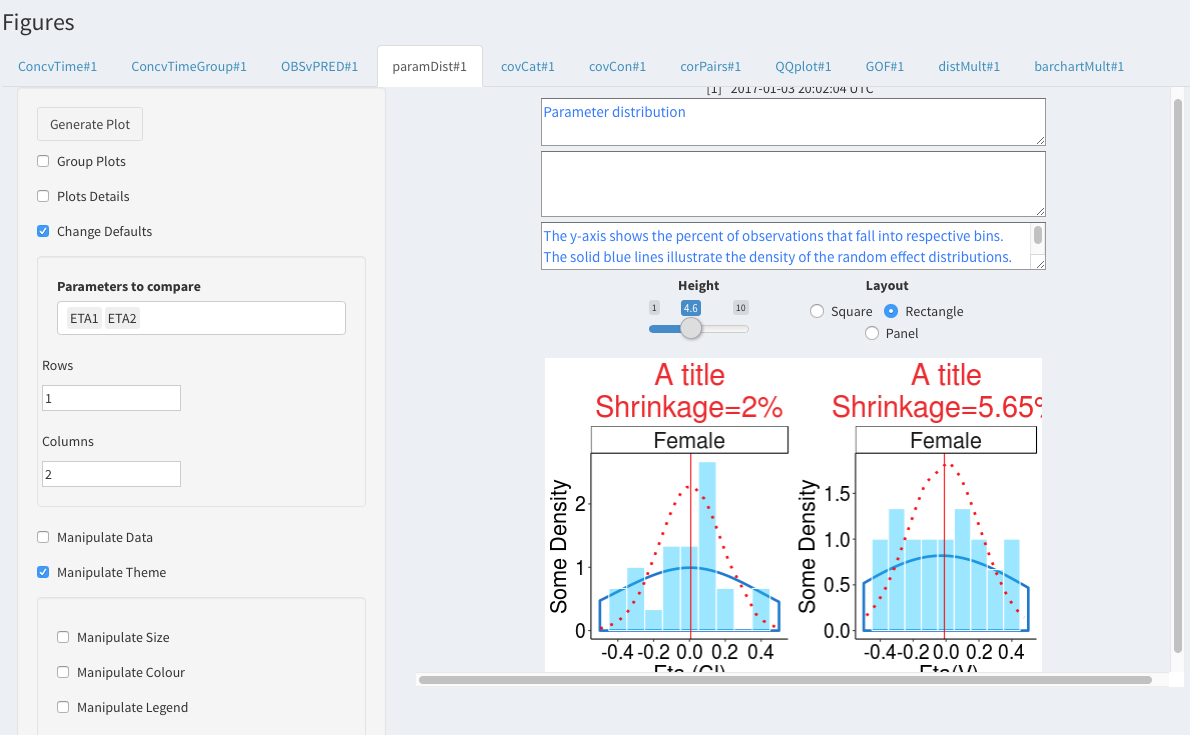
\includegraphics[width=.8\textwidth]{screencaps/04-06-1.png}
\caption{RID: 04 Test ID: 06 IDNum: 1}
\end{figure}
\begin{figure}[H]
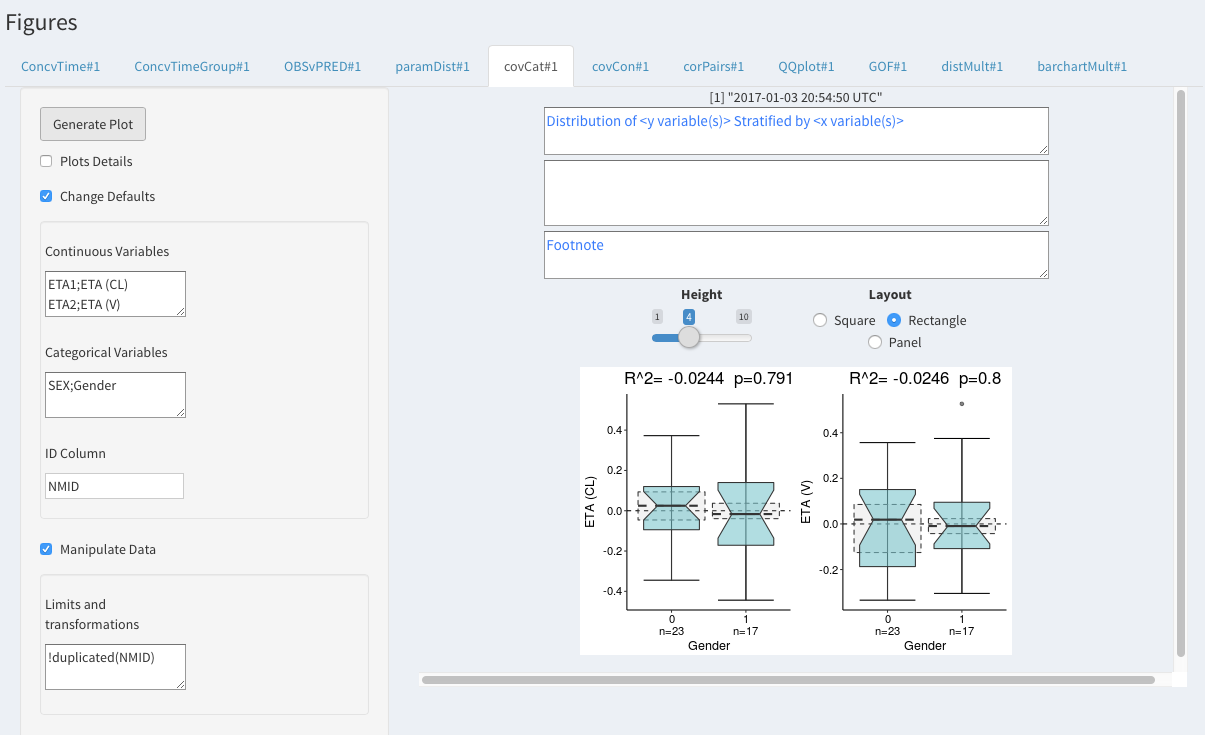
\includegraphics[width=.8\textwidth]{screencaps/05-01-1.png}
\caption{RID: 05 Test ID: 01 IDNum: 1}
\end{figure}
\begin{figure}[H]
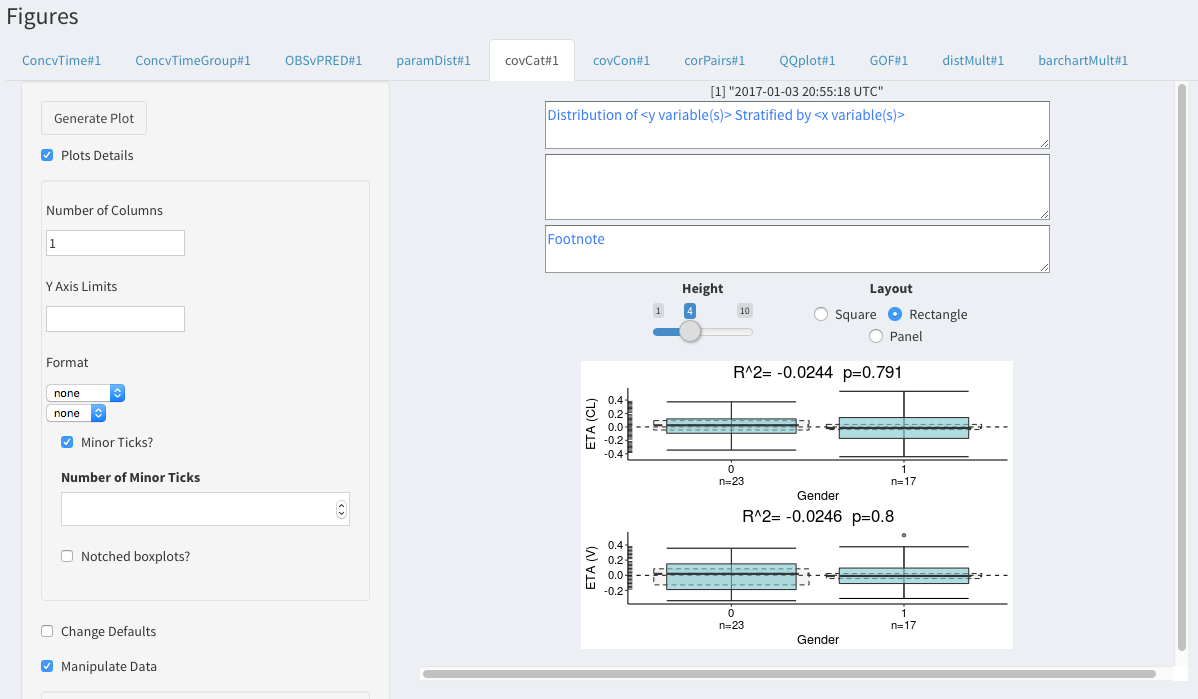
\includegraphics[width=.8\textwidth]{screencaps/05-02-1.png}
\caption{RID: 05 Test ID: 02 IDNum: 1}
\end{figure}
\begin{figure}[H]
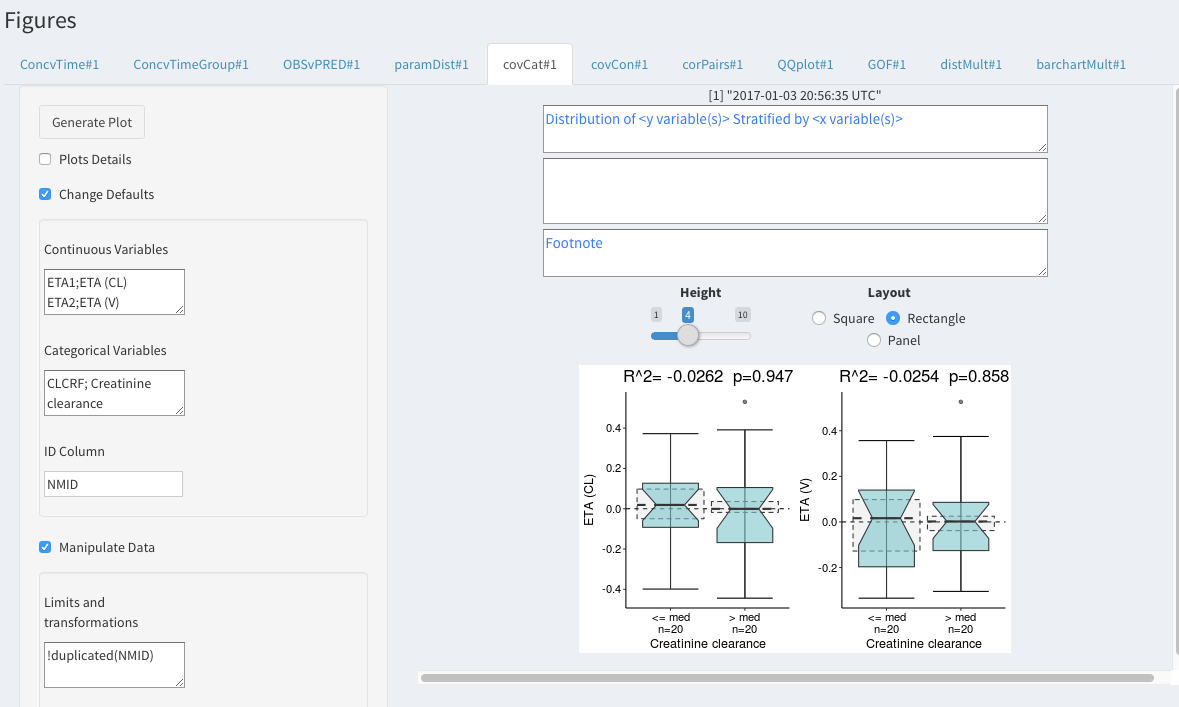
\includegraphics[width=.8\textwidth]{screencaps/05-03-1.png}
\caption{RID: 05 Test ID: 03 IDNum: 1}
\end{figure}
\begin{figure}[H]
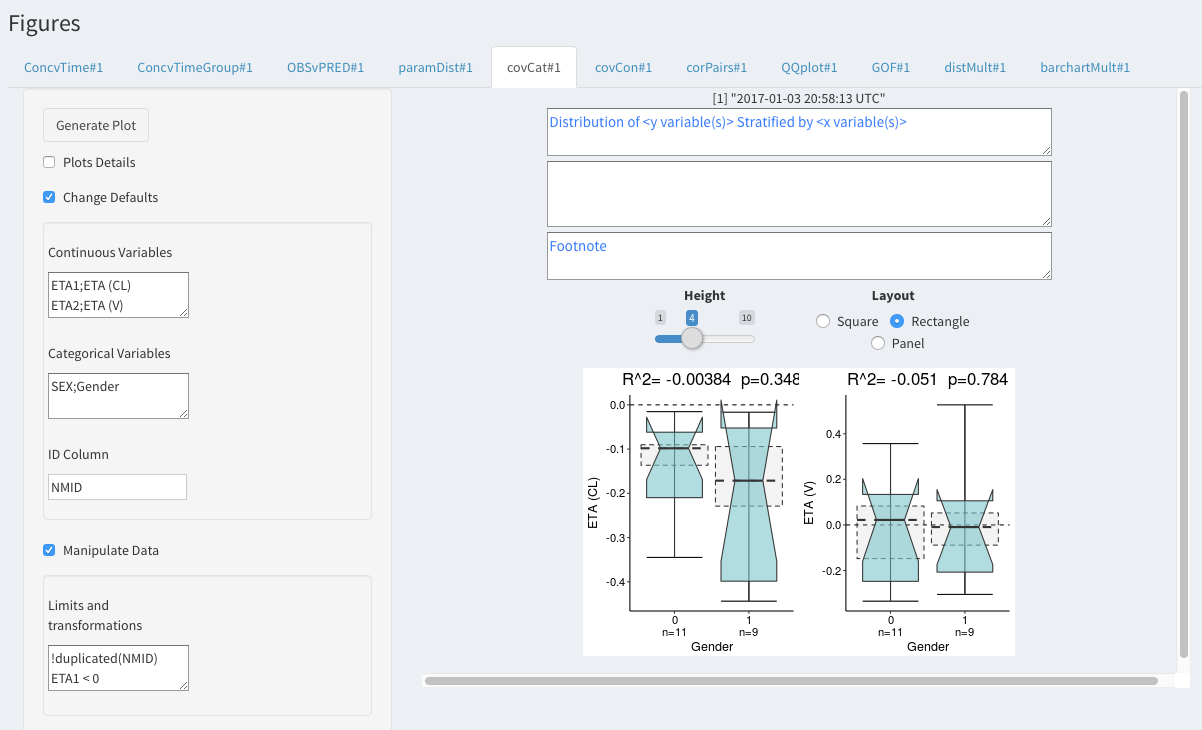
\includegraphics[width=.8\textwidth]{screencaps/05-04-1.png}
\caption{RID: 05 Test ID: 04 IDNum: 1}
\end{figure}
\begin{figure}[H]
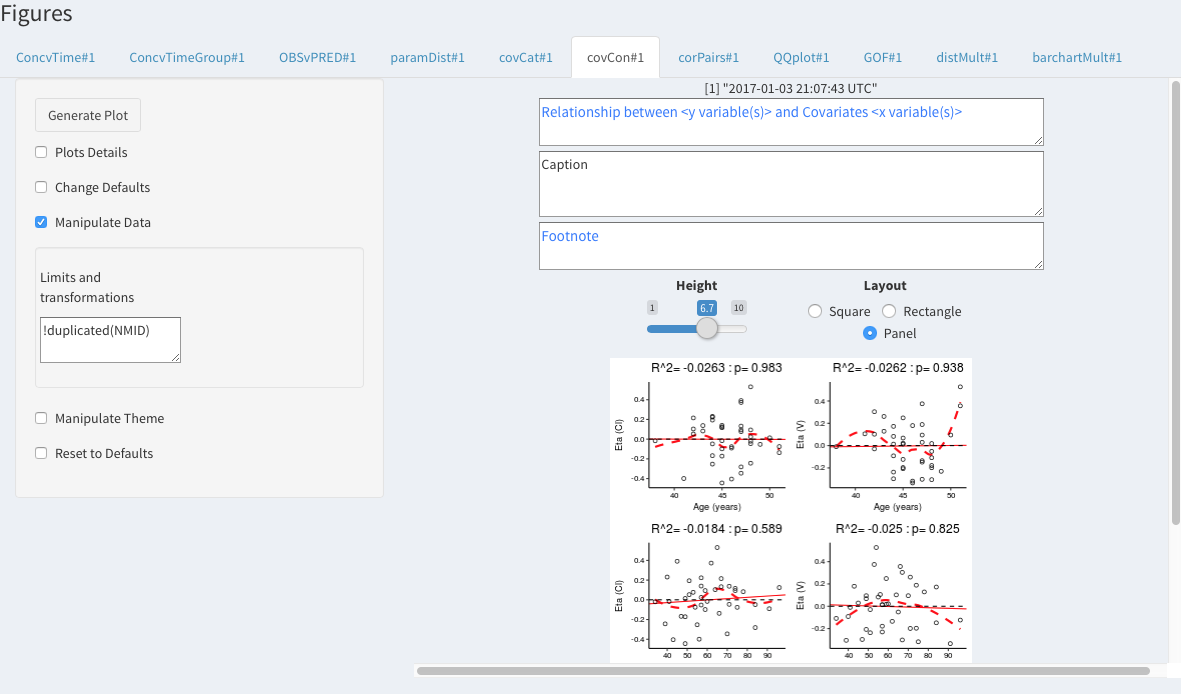
\includegraphics[width=.8\textwidth]{screencaps/06-01-1.png}
\caption{RID: 06 Test ID: 01 IDNum: 1}
\end{figure}
\begin{figure}[H]
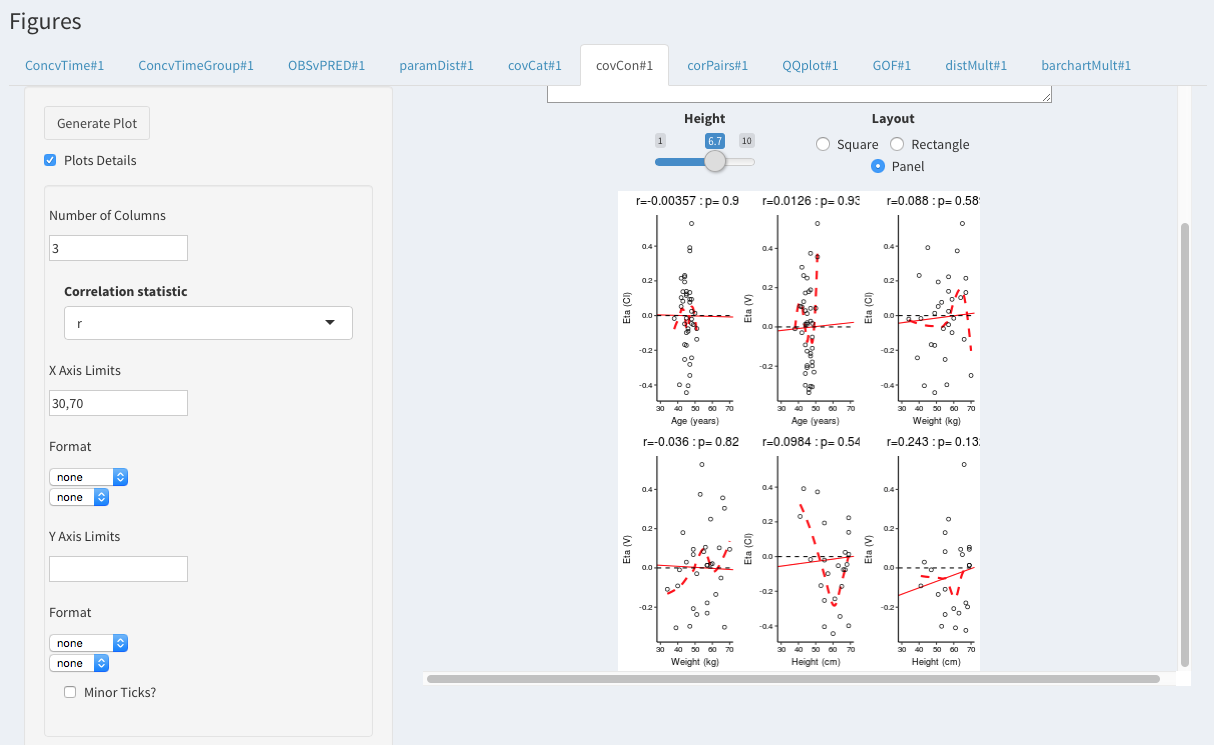
\includegraphics[width=.8\textwidth]{screencaps/06-02-1.png}
\caption{RID: 06 Test ID: 02 IDNum: 1}
\end{figure}
\begin{figure}[H]
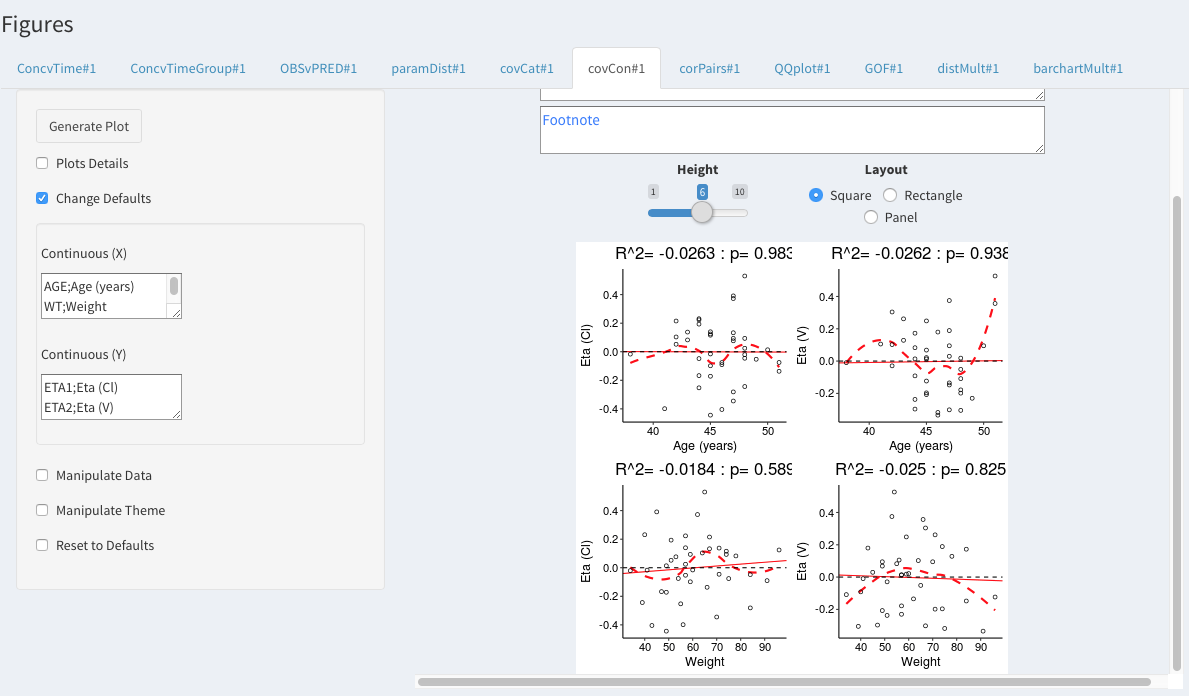
\includegraphics[width=.8\textwidth]{screencaps/06-03-1.png}
\caption{RID: 06 Test ID: 03 IDNum: 1}
\end{figure}
\begin{figure}[H]
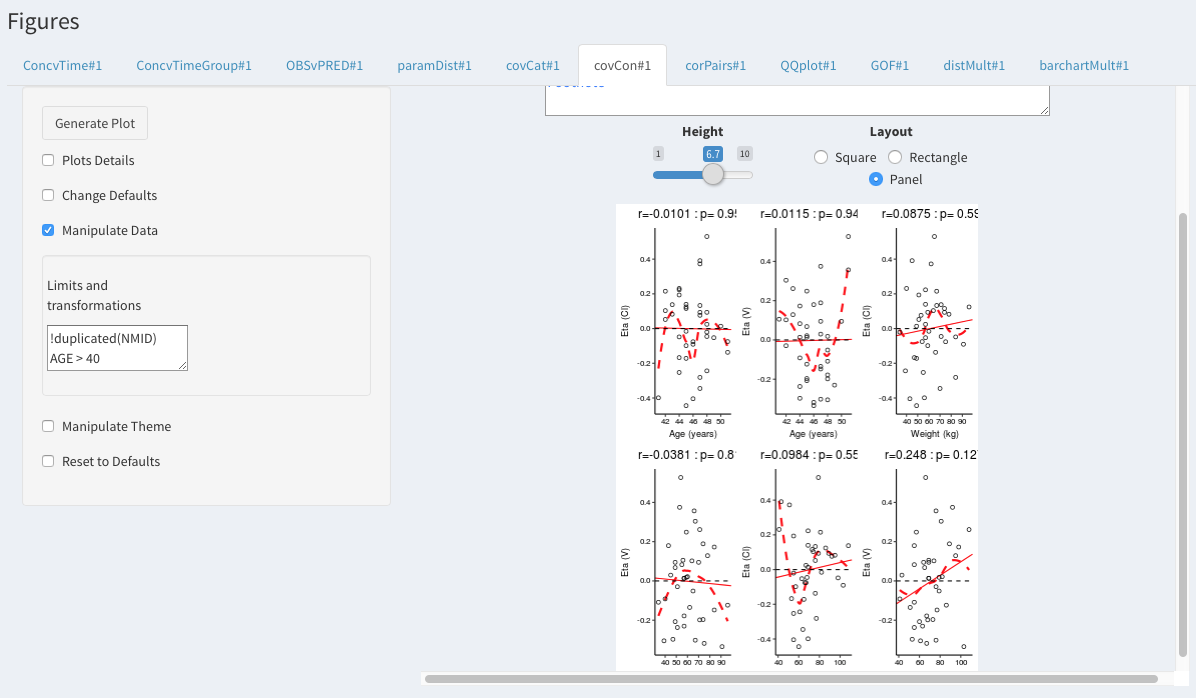
\includegraphics[width=.8\textwidth]{screencaps/06-04-1.png}
\caption{RID: 06 Test ID: 04 IDNum: 1}
\end{figure}
\begin{figure}[H]
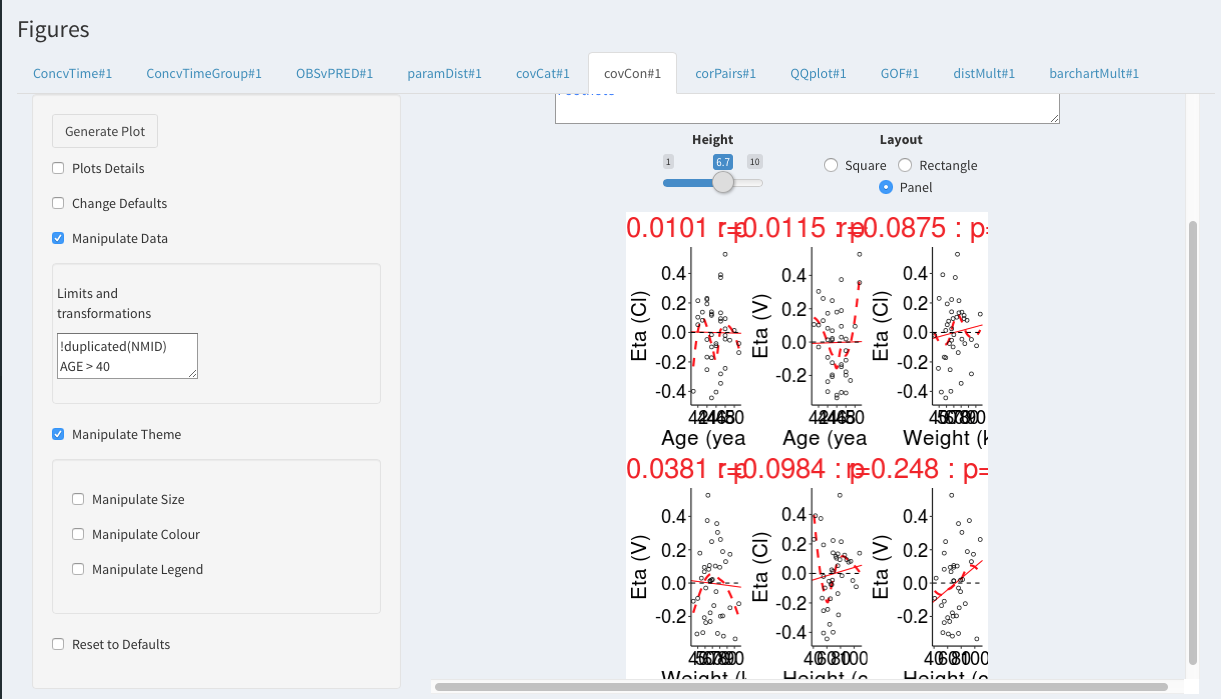
\includegraphics[width=.8\textwidth]{screencaps/06-05-1.png}
\caption{RID: 06 Test ID: 05 IDNum: 1}
\end{figure}
\begin{figure}[H]
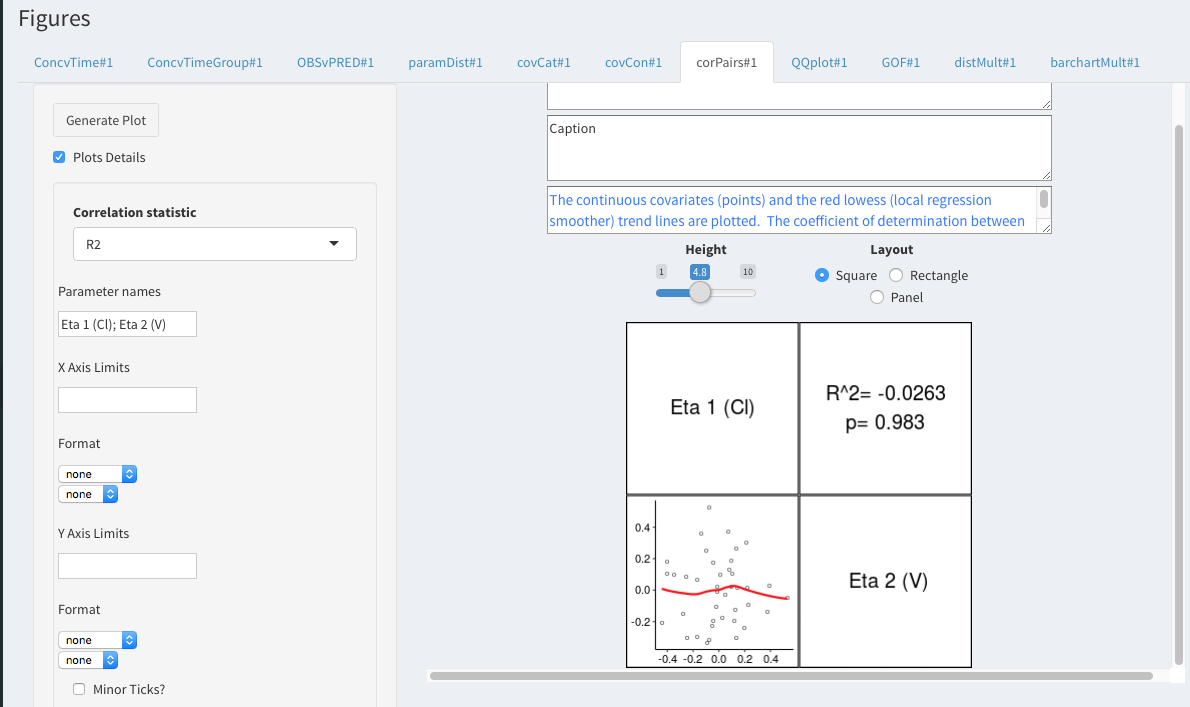
\includegraphics[width=.8\textwidth]{screencaps/07-01-1.png}
\caption{RID: 07 Test ID: 01 IDNum: 1}
\end{figure}
\begin{figure}[H]
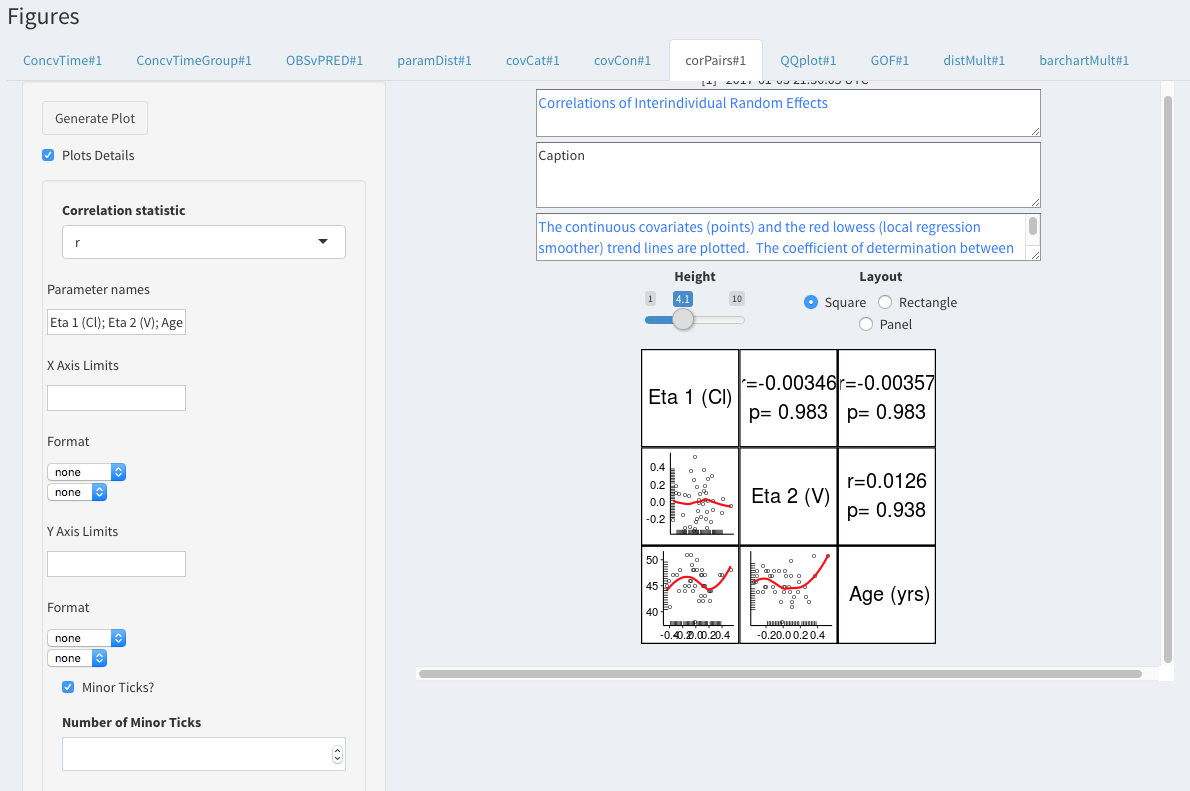
\includegraphics[width=.8\textwidth]{screencaps/07-02-1.png}
\caption{RID: 07 Test ID: 02 IDNum: 1}
\end{figure}
\begin{figure}[H]
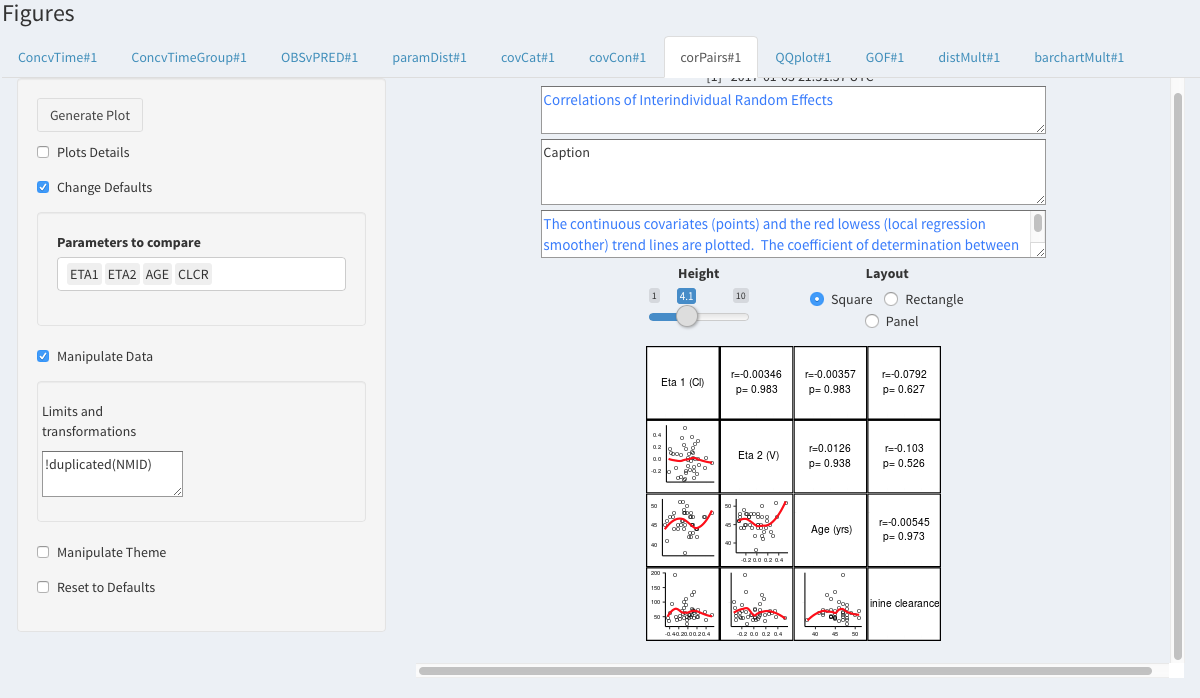
\includegraphics[width=.8\textwidth]{screencaps/07-03-1.png}
\caption{RID: 07 Test ID: 03 IDNum: 1}
\end{figure}
\begin{figure}[H]
\includegraphics[width=.8\textwidth]{screencaps/07-04-1.png}
\caption{RID: 07 Test ID: 04 IDNum: 1}
\end{figure}
\begin{figure}[H]
\includegraphics[width=.8\textwidth]{screencaps/07-05-1.png}
\caption{RID: 07 Test ID: 05 IDNum: 1}
\end{figure}
\begin{figure}[H]
\includegraphics[width=.8\textwidth]{screencaps/08-01-1.png}
\caption{RID: 08 Test ID: 01 IDNum: 1}
\end{figure}
\begin{figure}[H]
\includegraphics[width=.8\textwidth]{screencaps/08-02-1.png}
\caption{RID: 08 Test ID: 02 IDNum: 1}
\end{figure}
\begin{figure}[H]
\includegraphics[width=.8\textwidth]{screencaps/08-03-1.png}
\caption{RID: 08 Test ID: 03 IDNum: 1}
\end{figure}
\begin{figure}[H]
\includegraphics[width=.8\textwidth]{screencaps/08-04-1.png}
\caption{RID: 08 Test ID: 04 IDNum: 1}
\end{figure}
\begin{figure}[H]
\includegraphics[width=.8\textwidth]{screencaps/08-05-1.png}
\caption{RID: 08 Test ID: 05 IDNum: 1}
\end{figure}
\begin{figure}[H]
\includegraphics[width=.8\textwidth]{screencaps/08-06-1.png}
\caption{RID: 08 Test ID: 06 IDNum: 1}
\end{figure}
\begin{figure}[H]
\includegraphics[width=.8\textwidth]{screencaps/09-01-1.png}
\caption{RID: 09 Test ID: 01 IDNum: 1}
\end{figure}
\begin{figure}[H]
\includegraphics[width=.8\textwidth]{screencaps/09-02-1.png}
\caption{RID: 09 Test ID: 02 IDNum: 1}
\end{figure}
\begin{figure}[H]
\includegraphics[width=.8\textwidth]{screencaps/09-03-1.png}
\caption{RID: 09 Test ID: 03 IDNum: 1}
\end{figure}
\begin{figure}[H]
\includegraphics[width=.8\textwidth]{screencaps/09-04-1.png}
\caption{RID: 09 Test ID: 04 IDNum: 1}
\end{figure}
\begin{figure}[H]
\includegraphics[width=.8\textwidth]{screencaps/09-05-1.png}
\caption{RID: 09 Test ID: 05 IDNum: 1}
\end{figure}
\begin{figure}[H]
\includegraphics[width=.8\textwidth]{screencaps/09-06-1.png}
\caption{RID: 09 Test ID: 06 IDNum: 1}
\end{figure}
\begin{figure}[H]
\includegraphics[width=.8\textwidth]{screencaps/09-07-1.png}
\caption{RID: 09 Test ID: 07 IDNum: 1}
\end{figure}
\begin{figure}[H]
\includegraphics[width=.8\textwidth]{screencaps/09-08-1.png}
\caption{RID: 09 Test ID: 08 IDNum: 1}
\end{figure}
\begin{figure}[H]
\includegraphics[width=.8\textwidth]{screencaps/09-09-1.png}
\caption{RID: 09 Test ID: 09 IDNum: 1}
\end{figure}
\begin{figure}[H]
\includegraphics[width=.8\textwidth]{screencaps/09-10-1.png}
\caption{RID: 09 Test ID: 10 IDNum: 1}
\end{figure}
\begin{figure}[H]
\includegraphics[width=.8\textwidth]{screencaps/09-11-1.png}
\caption{RID: 09 Test ID: 11 IDNum: 1}
\end{figure}
\begin{figure}[H]
\includegraphics[width=.8\textwidth]{screencaps/09-12-1.png}
\caption{RID: 09 Test ID: 12 IDNum: 1}
\end{figure}
\begin{figure}[H]
\includegraphics[width=.8\textwidth]{screencaps/10-01-1.png}
\caption{RID: 10 Test ID: 01 IDNum: 1}
\end{figure}
\begin{figure}[H]
\includegraphics[width=.8\textwidth]{screencaps/10-02-1.png}
\caption{RID: 10 Test ID: 02 IDNum: 1}
\end{figure}
\begin{figure}[H]
\includegraphics[width=.8\textwidth]{screencaps/10-03-1.png}
\caption{RID: 10 Test ID: 03 IDNum: 1}
\end{figure}
\begin{figure}[H]
\includegraphics[width=.8\textwidth]{screencaps/10-04-1.png}
\caption{RID: 10 Test ID: 04 IDNum: 1}
\end{figure}
\begin{figure}[H]
\includegraphics[width=.8\textwidth]{screencaps/11-01-1.png}
\caption{RID: 11 Test ID: 01 IDNum: 1}
\end{figure}
\begin{figure}[H]
\includegraphics[width=.8\textwidth]{screencaps/11-02-1.png}
\caption{RID: 11 Test ID: 02 IDNum: 1}
\end{figure}
\begin{figure}[H]
\includegraphics[width=.8\textwidth]{screencaps/11-03-1.png}
\caption{RID: 11 Test ID: 03 IDNum: 1}
\end{figure}
\begin{figure}[H]
\includegraphics[width=.8\textwidth]{screencaps/11-04-1.png}
\caption{RID: 11 Test ID: 04 IDNum: 1}
\end{figure}
\begin{figure}[H]
\includegraphics[width=.8\textwidth]{screencaps/12-01-1.png}
\caption{RID: 12 Test ID: 01 IDNum: 1}
\end{figure}
\begin{figure}[H]
\includegraphics[width=.8\textwidth]{screencaps/12-02-1.png}
\caption{RID: 12 Test ID: 02 IDNum: 1}
\end{figure}
\begin{figure}[H]
\includegraphics[width=.8\textwidth]{screencaps/12-03-1.png}
\caption{RID: 12 Test ID: 03 IDNum: 1}
\end{figure}
\begin{figure}[H]
\includegraphics[width=.8\textwidth]{screencaps/12-03-2.png}
\caption{RID: 12 Test ID: 03 IDNum: 2}
\end{figure}
\begin{figure}[H]
\includegraphics[width=.8\textwidth]{screencaps/12-03-4.png}
\caption{RID: 12 Test ID: 03 IDNum: 4}
\end{figure}
\begin{figure}[H]
\includegraphics[width=.8\textwidth]{screencaps/12-03-5.png}
\caption{RID: 12 Test ID: 03 IDNum: 5}
\end{figure}
\begin{figure}[H]
\includegraphics[width=.8\textwidth]{screencaps/12-03-6.png}
\caption{RID: 12 Test ID: 03 IDNum: 6}
\end{figure}
\begin{figure}[H]
\includegraphics[width=.8\textwidth]{screencaps/12-04-1.png}
\caption{RID: 12 Test ID: 04 IDNum: 1}
\end{figure}
\begin{figure}[H]
\includegraphics[width=.8\textwidth]{screencaps/12-04-2.png}
\caption{RID: 12 Test ID: 04 IDNum: 2}
\end{figure}
\begin{figure}[H]
\includegraphics[width=.8\textwidth]{screencaps/12-04-3.png}
\caption{RID: 12 Test ID: 04 IDNum: 3}
\end{figure}
\begin{figure}[H]
\includegraphics[width=.8\textwidth]{screencaps/12-04-4.png}
\caption{RID: 12 Test ID: 04 IDNum: 4}
\end{figure}
\begin{figure}[H]
\includegraphics[width=.8\textwidth]{screencaps/12-04-5.png}
\caption{RID: 12 Test ID: 04 IDNum: 5}
\end{figure}
\begin{figure}[H]
\includegraphics[width=.8\textwidth]{screencaps/12-04-6.png}
\caption{RID: 12 Test ID: 04 IDNum: 6}
\end{figure}
\begin{figure}[H]
\includegraphics[width=.8\textwidth]{screencaps/12-05-1.png}
\caption{RID: 12 Test ID: 05 IDNum: 1}
\end{figure}
\begin{figure}[H]
\includegraphics[width=.8\textwidth]{screencaps/12-05-2.png}
\caption{RID: 12 Test ID: 05 IDNum: 2}
\end{figure}
\begin{figure}[H]
\includegraphics[width=.8\textwidth]{screencaps/12-05-3.png}
\caption{RID: 12 Test ID: 05 IDNum: 3}
\end{figure}
\begin{figure}[H]
\includegraphics[width=.8\textwidth]{screencaps/12-05-4.png}
\caption{RID: 12 Test ID: 05 IDNum: 4}
\end{figure}
\begin{figure}[H]
\includegraphics[width=.8\textwidth]{screencaps/12-05-5.png}
\caption{RID: 12 Test ID: 05 IDNum: 5}
\end{figure}
\begin{figure}[H]
\includegraphics[width=.8\textwidth]{screencaps/12-05-6.png}
\caption{RID: 12 Test ID: 05 IDNum: 6}
\end{figure}
\begin{figure}[H]
\includegraphics[width=.8\textwidth]{screencaps/12-06-1.png}
\caption{RID: 12 Test ID: 06 IDNum: 1}
\end{figure}
\begin{figure}[H]
\includegraphics[width=.8\textwidth]{screencaps/12-06-2.png}
\caption{RID: 12 Test ID: 06 IDNum: 2}
\end{figure}
\begin{figure}[H]
\includegraphics[width=.8\textwidth]{screencaps/12-06-3.png}
\caption{RID: 12 Test ID: 06 IDNum: 3}
\end{figure}
\begin{figure}[H]
\includegraphics[width=.8\textwidth]{screencaps/12-06-4.png}
\caption{RID: 12 Test ID: 06 IDNum: 4}
\end{figure}
\begin{figure}[H]
\includegraphics[width=.8\textwidth]{screencaps/12-06-5.png}
\caption{RID: 12 Test ID: 06 IDNum: 5}
\end{figure}
\begin{figure}[H]
\includegraphics[width=.8\textwidth]{screencaps/12-08-1.png}
\caption{RID: 12 Test ID: 08 IDNum: 1}
\end{figure}



%% \newpage
%%
%% \subsection*{Listings}
%%
%% {\bf RID: 2 Topic ID: 4}
%%
%% \verbatiminput{listings/asRootpkgSetup.Rout}
%%
%% \newpage
%% {\bf RID: 2 Topic ID: 5}
%%
%% \verbatiminput{listings/pkgSetup.Rout}
%%
\end{document}